\documentclass{report}

\usepackage{phdstyle}
\usepackage{RepSty}

\usepackage{setspace}

\usepackage[numbers]{natbib}

\newcommand{\bld}{\boldsymbol}
\newcommand{\Wx}{\Omega_x}
\newcommand{\Wy}{\Omega_y}
\newcommand{\Dt}{\Delta t}

% % Statistical requirements definitions
\newcommand{\td}{\mathrm{d}}
\newcommand{\pars}{\boldsymbol{\theta}}
\DeclareDocumentCommand{\Fisher}{O{}D(){\pars_0}}{I_{#1}(#2)}
\DeclareDocumentCommand{\Xpct}{mo}{\mathrm{E}\bkt*{#1\IfNoValueTF{#2}{}{|~ #2}}}
\DeclareDocumentCommand{\XpctO}{m}{\Xpct{#1}[\pars_0]}
\DeclareDocumentCommand{\mupp}{s}{\mu'_\phi\IfBooleanTF{#1}{}{(t_i)}}
\DeclareDocumentCommand{\mudpp}{s}{\mu''_{\phi^2}\IfBooleanTF{#1}{}{(t_i)}}
\newcommand{\vp}[2]{{#1}\cdot 10^{#2}}
\newcommand{\cnt}{c}
\newcommand{\meas}{\epsilon}
\newcommand{\dt}{\Delta t}
\newcommand{\dtm}{\dt_{\meas}}
\newcommand{\dtc}{\dt_{\cnt}}
\newcommand{\Ncm}{{n_{\sfrac{\cnt}{\meas}}}}
\newcommand{\Nmnd}{{n_{\sfrac{\meas}{zc}}}}
\newcommand{\Nnd}{{n_{zc}}}
\newcommand{\Nm}{{n_{\meas}}}
\newcommand{\Ncnt}{{n_{\cnt}}}
\newcommand{\LTb}{\tau_b}
\newcommand{\LTd}{\tau_d}
\newcommand{\lamb}{\lambda_b}
\newcommand{\lamd}{\lambda_d}

\newcommand{\home}{/Users/alexaksentyev}
\newcommand{\Artem}{\home/REPOS/COSYINF/img/Artem}
\newcommand{\multisext}{\Artem/multisext_test}
\newcommand{\compare}{\Artem/spin_vs_polarization_fit_comp}
\newcommand{\decoh}{\Artem/decoherence_frequency_dependence}

\begin{document}
\singlespacing
\begin{titlepage}

\begin{center}
{МИНИСТЕРСТВО ОБРАЗОВАНИЯ И НАУКИ РОССИЙСКОЙ ФЕДЕРАЦИИ}\\[3pt]
\textsc{\small{Федеральное государственное автономное образовательное учреждение высшего образования}}\\

\textbf{\enquote{Национальный исследовательский ядерный университет\\
{``МИФИ''}}}\\
\textbf{(НИЯУ МИФИ)}\\[2cm]




\textsc{\textbf{Отчет о научно-исследовательской деятельности\\		
		аспиранта и подготовке научно-квалификационной\\	
		работы (диссертации) на соискание ученой степени\\		
		кандидата наук за первое полугодие 4 курса}}\\[2cm]

% Title
\enquote{Исследование магнитооптических структур со свойствами замороженного и квази-замороженного спина для поиска электрического дипольного момента дейтрона в накопительном кольце}\\[2cm]


\end{center}


\begin{flushleft}
% Author and supervisor
\begin{tabular}{ll}
	Аспирант                   & А.Е. Аксентьев                           \\
	Направление                & 03.06.01 Физика и астрономия             \\
	Научная специальность      & 01.04.20 Физика пучков заряженных частиц \\
	                           & \-\hspace{1.8cm} и ускорительная техника \\[1cm]
	Научный руководитель       &                                          \\
	Должность, степень, звание & С.М. Полозов, к.ф.-м.н, доц.             \\%[1cm]
	                           & Ю.В. Сеничев, д.ф-м.н., проф.            \\[1cm]
	Дата защиты:               &                                          \\
	Результат защиты:          &
\end{tabular}

\end{flushleft}

\vfill


\begin{center}
Москва \the\year{}
\end{center}



\end{titlepage}


\tableofcontents 
\pagebreak

\onehalfspacing

\chapter{Постановка целей и задач исследования}

\section{Цели, задачи, перспективы исследования}\label{sec:research_program}

Целью исследования является сравнение структур с Замороженным и Квази-замороженным спином, для определения которая из них больше подходит для проведения эксперимента по поиску ЭДМ дейтрона с точностью $10^{-29}$ e$\cdot$cm.

Для достижения поставленной цели предложена следующая программа:
\begin{enumerate}
\item Анализ требований к эксперименту по поиску дейтронного ЭДМ методом определения частоты прецессии спина, обоснованных статистическими соображениями;
\item Изучение влияния неточности установки E+B спин-ротаторов на систематическую ошибку определения частоты ЭДМ прецессии (фальш-сигнал);
\item Изучение явления деполяризации пучка засчёт эффекта декогеренции спин-тюна, а также его подавление при помощи секступольных полей в неидеальной структуре;
\item Изучение влияния нарушения спин-прецессии на конечную статистику в частотном методе определения ЭДМ;
\item Моделирование процедуры калибровки ведущего магнитного поля кольца для его точного обращения при обратной инжекции пучка в процедуре CW/CCW.
\end{enumerate}

В перспективе предполагается использование предложенного метода поиска ЭДМ элементарной частицы в частотной области, а также разработанной в рамках данной работы методологии анализа колец, при конструировании кольца по поиску дейтронного ЭДМ на комплексе НИКА, Дубна.

\section{Актуальность и научная новизна работы}

\subsection{Актуальность}

Вся наблюдаемая вселенная состоит преимущественно из материи; антиматерия может быть получена в ускорителях заряженных частиц, но в пренебрежимо малых количествах. На сегодняшний день считается, что вскоре после Большого Взрыва материя была образована из энергии в парах частица-античастица, после чего последовала стадия аннигиляции; однако, по какой-то причине, эта фаза закончилась превалированием материи над антиматерией (по крайней мере в наблюдаемой вселенной) --- процесс называемый \emph{бариогенезом.}

В 1967 году, академик АН СССР Андрей Сахаров определил условия, требуемые для бариогенеза (независимо от механизма его действия). Одно из \emph{условий Сахарова} --- существование процессов, нарушающих C- и CP-симметрии. Известны источники нарушения этих симметрий, однако их не достаточно для объяснения барионной асимметрии вселенной; поиск продолжается.

Интерес поиска Электрического Дипольного Момента (ЭДМ) элементарных частиц состоит в том, что, если они существуют, то они нарушают P- и T-симметрии. Таким образом, обнаружение ненулевых ЭДМ элементарных частиц может привести нас к физике за границами Стандартной Модели; такие теории как SUSY (суперсимметрия) указывают на наличие ЭДМ гораздо большей величины (на уровне $10^{-29} - 10^{-24}$ e$\cdot$cm), чем предсказывает Стандартная Модель.

\subsection{Новизна}

В данной работе исследуется возможность измерения электрического
дипольного момента дейтрона с помощью накопительного кольца,
построенного на основе принципа Замороженного (или
Квази-замороженного) спина, методом Frequency Domain.

Разработкой метода Frequency Domain занимается проф. Ю. Сеничев в
рамках коллаборации JEDI Исследовательского центра ``Юлих. ''
Frequency Domain Method (далее FDM) базируется на концепциях замороженного спина,
впервые предложенной в 2008 году коллаборацией Брукхейвенской
Национальной Лаборатории, и Spin Wheel, предложенной профессором И. Коопом
(Новосибирский Государственный Университет) в 2012. Однако ни тот, ни другой
метод сам по себе не решают проблему неточности установки элементов
ускорителя, и возникающий в связи с этим фальш-сигнал.  На сегодняшний
день, FDM --- это единственный известный,
практически-реализуемый метод, решающий данную проблему.

\section{Структура работы}
Структура работы следует пунктам программы обозначенной в разделе~\ref{sec:research_program}

\chapter{Характеристика современного состояния изучаемой проблемы}
Поиск ЭДМ в невырожденных системах был инициирован Эдвардом Пёрселлом
и Норманом Рэмзи более 50 лет назад, для нейтрона. С тех пор было
проведено множество всё более чувствительных экспериментов на
нейтронах, атомах, и молекулах, и тем не менее, ЭДМ пока ещё не был
обнаружен. На данный момент, верхний предел ЭДМ нейтрона оценивается
на уровне $<3\cdot 10^{-26}$ e$\cdot$cm, протона --- $<8\cdot
10^{-25}$ e$\cdot$cm.~\citep[стр.~9]{Pretz:Presentation}

В 2008 году коллаборацией в Брукхейвенской Национальной Лаборатории (BNL, США) был предложен эксперимент по измерению ЭДМ дейтрона, основанный на использовании эффекта замороженного спина в магнитном накопительном кольце.~\cite{BNL:Deuteron2008} 

В 2015 году, коллаборацией Storage Ring EDM Collaboration, был предложен эксперимент по поиску протонного ЭДМ в полностью электрическом накопительном кольце.~\cite{BNL:Proton}

На данный момент, коллаборацией JEDI (Исследовательский центр ``Юлих,'' Германия) ведётся разработка структуры накопительного кольца для проведения предварительного эксперимента по измерению дейтронного ЭДМ на полностью магнитном синхротроне COSY. В рамках исследований, проводимых коллаборацией, была выдвинута концепция квази-замороженного кольца. Также, профессором Ю. Сеничевым была предложена методология поиска ЭДМ в частотной области (так называемый Frequency Domain Method).

\section{BNL FS (Frozen Spin) концепция}
\subsection{Уравнение Т-БМТ}
Уравнение Томаса-БМТ описывает динамику спин-вектора $\vec s$ в
магнитном поле $\vec B$ и электростатическом поле $\vec E$. Его
обобщённая версия, включающая влияние ЭДМ, может быть записана (в
системе центра масс пучка) как:~\cite[стр.~6]{Eremey:Thesis}
\begin{subequations}
  \begin{align}
    \ddt{\vec s} &= \vec s\times \bkt{\vec\W_{MDM} +\vec\W_{EDM}}, \label{eq:TBMT_main}
    \intertext{где МДМ и ЭДМ угловые скорости $\vec\W_{MDM}$ и $\vec\W_{EDM}$ }
    \vec\W_{MDM} &= \frac qm \bkt*{G\vec B - \bkt{G - \frac{1}{\gamma^2-1}}\frac{\vec E\times\vec\beta}{c}},\label{eq:TBMT_MDM} \\
    \vec\W_{EDM} &= \frac qm \frac\eta2 \bkt*{\frac{\vec E}c + \vec\beta\times \vec B}.\label{eq:TBMT_EDM}
  \end{align}
\end{subequations}
В уравнениях выше, $m,~q,~G=(g-2)/2$ есть, соответственно, масса, заряд, и
магнитная аномалия частицы; $\beta = \sfrac{v_0}{c}$,
нормализованная скорость частицы; $\gamma$ её Лоренц-фактор. ЭДМ
множитель $\eta$ определяется уравнением $d = \eta\frac{q}{2mc}s$, где
$d$ --- ЭДМ частицы, а $s$ её спин.

\subsection{Концепция замороженного спина}
Из уравнения~\eqref{eq:TBMT_MDM} можно видеть, что, в отсутствии ЭДМ,
направление вектора спина частицы пучка может быть зафиксировано
относительно её вектора импульса: $\vec\W_{MDM}=\vec 0$; иными словами, можно реализовать
условие замороженности спина (Frozen Spin condition).

Достоинством налагания FS-условия на пучок в накопительном кольце
следующее: в соответствии с
уравнениями~\cref{eq:TBMT_main,eq:TBMT_MDM,eq:TBMT_EDM}, векторы МДМ и
ЭДМ угловых скоростей ортогональны, а потому в общей скорости
прецессии они складываются квадратично, в связи с чем сдвиг частоты
прецессии, связанный с ЭДМ, становится эффектом второго порядка
величины:~\citep[стр.~5]{Mane:SpinWheel}
\[
\w \propto \sqrt{\W_{MDM}^2 + \W_{EDM}^2} \approx \W_{MDM} + \frac{\W_{EDM}^2}{2\W_{MDM}}.
\]
Это обстоятельство значительно ухудшает чувствительность эксперимента.

Однако, заморозив спин в горизонтальной плоскости, единственная
осающаяся МДМ компонента угловой скорости сонаправлена с ЭДМ
компонентой, а значит складывается с ней линейно. Таким образом,
чувствительность значительно улучшается.

\subsection{Реализация условия замороженности спина в накопительном кольце}
Накопительные кольца могут быть классифицированы в три группы:
\begin{enumerate}
\item чисто магнитные (как COSY, NICA, etc),
\item чисто электростатические (Brookhaven AGS Analog Ring),
\item комбинированные.
\end{enumerate}

Ввиду уравнения~\eqref{eq:TBMT_MDM}, условие FS не может быть
выполнено в чисто магнитном кольце.

Для некоторого числа частиц, таких как протон, чья $G>0$, чисто
электростатическое кольцо может быть использовано в рамках FS
методологии ЭДМ эксперимента с пучком на так называемой ``магической''
энергии, определяемой как $\gamma_{mag} = \sqrt{(1+G)/G}$.

Для частиц с $G<0$ (таких как дейтрон),это невозможно, и необходимо
использовать комбинированное кольцо. Для того, чтобы реализовать FS
условие в комбинированном кольце, вводится ~\cite{BNL:Deuteron2008} радиальное электрическое
поле величины
\begin{equation}\label{eq:FS_Er}
  E_r = \frac{GB_yc\beta\gamma^2}{1-G\beta^2\gamma^2}.
\end{equation}

\subsection{BNL FS метод}\label{sec:BNLFS_concept}
BNL FS метод, предложенный коллаборацией, занимающейся разработкой
метода измерения ЭДМ в накопительном кольце в Брукхейвенской
Национальной Лаборатории (США) в 2008 году,~\cite{BNL:Deuteron2008}
это метод для комбинированного кольца. Пучок продольно-поляризованных
дейтронов инжектируется в кольцо; с помощью поляриметрии наблюдается
его спин-прецессияв вертикальной и горизонтальной плоскостях; ЭДМ
сигнал --- это изменение вертикальной компоненты поляризации со
временем, выражаемое как:~\citep[стр.~8]{BNL:Deuteron2008}
\begin{equation}
  \Delta P_V = P\frac{\w_{edm}}{\W}\sin\bkt{\W t + \Theta_0},
\end{equation}
где $\W = \sqrt{\w_{edm}^2 + \w_a^2}$, $\w_a,~\w_{edm}$ угловые
скорости вызываемые, соответственно, магнитным и электрическим
дипольными моментами.

Налагая радиальное магнитное поле $E_r$~\eqref{eq:FS_Er}, ожидается
уменьшение компоненты $\w_a$ по крайней мере на фактор $10^9$; ввиду
малости величины гипотезируемой $\w_{edm}$, $\Delta P_V \approx P
\w_{edm} t$, и максимальная величина $\Delta P_V$ возрастает в $10^9$.

Ожидаемая чувствительность эксперимента $10^{-29}~e\cdot cm$ за $10^7$
секунд (6 месяцев) полного времени измерения. На этом уровне
чувствительности, асимметрия сечения $\varepsilon_{LR} \approx 5\cdot
10^{-6}$ для наименьших практически реализуемых значений
$\w_a$.~\citep[стр.~18]{BNL:Deuteron2008} Последнее обстоятельство
ставит серьёзную проблему для поляриметрии.~\cite{Mane:SpinWheel} Один
из вариантов её решения лежит в применении внешнего радиального
магнитного поля и измерении обзей частоты прецессии засчёт МДМ и ЭДМ
вместе. Это основа так называемого метода Spin Wheel, о котором в
следующем разделе.

Единственный известный систематический эффект спиновой динамики
первого порядка это присутствие ненулевой средней вертикальной
компоненты электрического поля $\avg{E_V}$. В этом случае, спин будет
прецессировать вокруг радиального направления с частотой~\citep[стр.~11]{BNL:Deuteron2008}
\[
\w_{syst} \approx \frac{\mu\avg{E_V}}{\beta c\gamma^2}.
\]
Здесь важно рассмотреть два обстоятельства:
\begin{itemize}
\item присутствие $\avg{E_V}\neq 0$ вызвано ошибкой юстировки
  элементов ускорителя;
\item этот систематический эффект меняет знак при инжекции пучка в
  обратном направлении.
\end{itemize}
Последнее обстоятельство является причиной структуры инжекции пучка
использованной в этом методе (сначала по-часовой, потом
против-часовой; CW/CCW). Хотя $\w_{syst}$ меняет знак при смене
направления движения пучка , эта методология тем не менее не учитывает
его \emph{величину}. В разделах~\ref{sec:SystErr:FakeSignalSim} и~\ref{sec:FalseSignalSim}, мы
показываем, что при реалистичной величине ошибки установки
спин-ротаторов 100 мкм, частота МДМ прецессии вокруг радиальной оси
находится на уровне 50--100 рад/сек.~\cite{Senichev:FDM} В связи с
этим, невозможно использовать данную методологию в её оригинальном варианте.

\section{Spin Wheel концепция}
Озвученные выше проблемы с поляриметрией и высокой скоростью прецессии
решаются в Spin Wheel (SW) модификации, предложенной проф. И. Коопом
(Новосибирский Государственный Университет). Основная идея метода в
следующем: сначала, обеспечивается условие замороженного спина; затем
включается радиальное магнитное поле величины $B_x$, достаточно сильное чтобы
вызвать вращение спина с частотой порядка 1 Гц. Поскольку поле
радиальное, вызванная им МДМ прецессия сонаправлена с ЭДМ, а значит
они складываются линейно: $\w \propto \W_{MDM} + \W_{EDM}$.

ЭДМ вклад вычисляется сравнением циклов с обратными знаками $B_x$:~\citep[стр.~1963]{Koop:IPAC13}
\[
\W_{EDM} = \frac{\W_x(+B_x) + \W_x(-B_x)}{2}.
\]

Внешнее поле также вызовет разделение орбит
пучков.~\citep[стр.~1963]{Koop:IPAC13} Это разделение может быть
измерено на уровне пико-метров SQUID магнетометрами; его предлагается
использовать для калибровки внешнего поля.

Поскольку из-за внешнего поля прецессия вокруг радиальной оси на 10
порядков выше чем в оригинальном предложении, значительно упрощается
задача для поляриметрии. Однако, существуют сомнения в возможности
измерить вызываемое внешним полем разделение орбит даже при помощи SQUIDов.

Также, проблема паразитного поля, вызванного ошибкой юстировки, не решена.

\section{Frequency Domain метод}\label{sec:FDM_concept}
Методология Frequency Domain (далее FDM)~\cite{Senichev:FDM} была разработана специально для решения проблемы неточности установки магнитов, и возникающего в связи с этим паразитного МДМ вращения спина. Как было обозначено выше, частота вращения спина в вертикальной плоскости, связанная с магнитным дипольным моментом, при реалистичной ошибке юстировки, находится на уровне 8--16 Гц, что делает невозможным наблюдение медленного нарастания вертикальной компоненты поляризации, связанное с наличием у частицы электрического дипольного момента, как предполагается оригинальным BNL FS методом. В FDM, ЭДМ-эффект вычисляется путём сравнения комбинированной (МДМ + ЭДМ) частоты прецессии, наблюдаемой при циркуляции пучка в прямом и обратном направлениях. Поскольку при смене полярности ведущего поля $\vec B \mapsto -\vec B$, $\vec\beta \mapsto -\vec\beta$, и $\vec E \mapsto \vec E$:
\begin{subequations}
  \begin{align}
    \w_x^{CW/CCW} &= \w_x^{MDM, CW/CCW} + \w_x^{EDM, CW/CCW}, \\
    \w_x^{MDM, CW} &= -\w_x^{MDM, CCW} \equiv \w_x^{MDM}, \label{eq:FDM_CW_CCW_MDM} \\
    \w_x^{EDM, CW} &= \w_x^{EDM, CCW} \equiv \w_x^{EDM},
    \intertext{поэтому, ЭДМ эстиматор}
    \hat\w_x^{EDM} &:= \frac12\bkt{\w_x^{CW} + \w_x^{CCW}} \label{eq:FDM_estimator} \\
                  &= \w_x^{EDM} + \underbrace{\frac12\bkt{\w_x^{MDM, CW} + \w_x^{MDM, CCW}}}_{\varepsilon \to 0}.
  \end{align}
\end{subequations}

Для того, чтобы гарантировать малость $\varepsilon$ по сравнению с требуемой точностью измерений, т.е., что уравнение~\eqref{eq:FDM_CW_CCW_MDM} выполняется достаточно точно, была разработана специальная процедура смены полярности ведущего поля, описанная в разделе~\ref{sec:Field_flipping}.

%% \section{Предварительный библиографический список по теме диссертации}
%% Диссертация Еремея Валетова.~\citep{Eremey:Thesis}
%% AGS Proposal (deuteron).
%% Senichev: Investigation of lattice for deuteron EDM ring.\\
%% Senichev: Spin tune decoherence effects in electro- and magnetostatic structures.
%% Senichev: Search for the charged particle electric dipole moments in storage rings.\\
%% Senichev: Frequency domain method of the search for the deuteron electric dipole moment in a storage ring with imperfections.
%% JEDI: Spin Tune mapping.


\chapter{Результаты разработки основных направлений теоретической концепции (FS и QFS колец)}
\section{Статистический анализ требований к эксперименту по поиску
  ЭДМ}

Вводные рассуждения по поводу измерения поляризации, проблемы
деполяризации пучка, и т.п.

\subsection{Модель частоты событий на поляриметре}
В наших рассуждениях мы предположили следующую простую модель
измеряемого сигнала:
\begin{equation}\label{eq:DetCntRt}
	N(t) = N_0(t)\cdot\bkt{1 + P\cdot e^{-\sfrac{t}{\LTd}}\cdot\sin(\omega\cdot t + \phi)},
\end{equation}
где $N_0(t)$ частота событий, связанная с неполяризованным сечением,
$\LTd$ время жизни поляризации, связанное с декогеренцией.

Ток пучка, рассеиваемого на мишени может быть описан с помощью:
\[
I(t)= I_0\cdot e^{t/\LTb} = \nu N_0^b\cdot e^{t/\LTb},
\]
где $\LTb$ --- время жизни пучка, $N_0^b$ его начальное число частиц,
и $\nu$ частота оборота пучка в ускорителе. Обозначая $p$ вероятность
что рассеянная частица полетит в сторону детектора, ожидаемое число
частиц, детектируемых в течении времени измерения $\dtc$ может быть
записано как
\begin{align}
N_0(t) & = p\cdot\int_{-\dtc/2}^{+\dtc/2} I(t+\tau)\td\tau \notag                    \\
& = p\cdot\frac{\nu N_0^b}{\lamb} e^{\lamb t}\cdot \bkt{e^{\lamb\sfrac{\dtc}{2}} - e^{-\lamb\sfrac{\dtc}{2}}} \notag \\
& \approx \underbrace{p\cdot\nu N_0^b e^{\lamb t}}_{\text{rate}~r(t)} \cdot\dtc.
\end{align}
Таким образом, получаем распределение Пуассона
\[
	P_{N_0(t)}(\tilde{N}_0) = \frac{\bkt{r(t)\dtc}^{\tilde{N}_0}}{\tilde{N}_0!}\cdot e^{-r(t)\dtc},
\]
с дисперсией $\SD{\tilde{N}_0}^2(t) = N_0(t)$. %In the limit of large $N_0(t)$, one can use the Gaussian approximation.

Нас интересует ожидаине $N_0(t) = \Xpct{\tilde{N}_0(t)}$, и его
стандартное отклонение $\SD{N_0}(t)$. Обозначая время измерения одного
события $\dtm$, полное время измерений $\dtc$, и число событий за
измерение $\Ncm = \dtm/\dtc$, ожидание
\begin{equation*}
	\Xpct{\tilde{N}_0(t)}_{\dtm} = \frac{1}{\Ncm}\sum_{i=1}^\Ncm \tilde{N}_0(t_i).
\end{equation*}
Поскольку это сумма случайных переменных, $N_0(t)$ имеет нормальное
распределение; тогда стандартное отклонение среднего % abuse of notation here (SD in place of SE) for aesthetic reasons
\begin{align*}
\SD{N_0}(t) & = \SD{\tilde{N}_0}(t)/\sqrt{\Ncm} = \sqrt{N_0(t)\frac{\dtc}{\dtm}}            \\
& \approx \sqrt{\frac{p\cdot\nu N_0^b}{\dtm}}\cdot\dtc \cdot\exp\bkt{\frac{\lamb}{2}\cdot t}.
\end{align*}
\newcommand{\A}{\frac{1}{\sqrt{p\cdot\nu N_0^b}}}

Отметим, что относительная ошибка растёт со временем:
\begin{equation}\label{eq:MeasRelErr}
	\frac{\SD{N_0}(t)}{N_0(t)} \approx \frac{A}{\sqrt{\dtm}}\cdot\exp\bkt{-\frac{\lamb}{2}t} = \frac{A}{\sqrt{\dtm}}\cdot\exp\bkt{\frac{t}{2\LTb}},~ A=\A.
\end{equation}

\subsection{Асимметрия сечения}
\newcommand{\Asym}{\mathcal{A}}
В качестве меры поляризации пучка используют асимметрию частоты
событий детекторов.~\citep[стр.~17]{Eversmann:Thesis} Асимметрия сечения
взаимодействия --- это нормализованная разность числа событий (в
единицу времени) на
детекторах, расположенных по разные стороны от вакуумной камеры:
\begin{equation}\label{eq:AsymDef}
	\Asym = \frac{N(\frac\pi2) - N(-\frac\pi2)}{N(\frac\pi2)+N(-\frac\pi2)}.
\end{equation}

В связи с уменьшением числа частиц в пучке, измерение асимметрии
сечения гетероскедастично. Из~\citep[стр.~18]{Eversmann}, мы приняли
модель гетероскедастичности
\begin{equation}\label{eq:AsymHtsk}
	\SD{\Asym}^2(t) \approx \frac{1}{2N_0(t)}.
\end{equation}

\subsection{Временное окно измерений}
\DeclareDocumentCommand{\stat}{s}{\IfBooleanTF{#1}{X_{tot}}{\frac{\SD{\meas}^2}{\SE{\hat\omega}^2\cdot \var[w]{t}}}}
\DeclareDocumentCommand{\var}{O{}mo}{\mathrm{var}_{#1}\bkt*{#2\IfValueT{#3}{\vert~ #3}}}
\newcommand{\dtnd}{\dt_{zc}}
\newcommand{\SNR}{\text{SNR}}

Предполагая нормальное распределение ошибки измерений, с нулевым
ожиданием и дисперсией $\SD{\meas}^2$, эстиматор максимального
правдоподобия дисперсии оценки частоты колебаний асимметрии сечения
взаимодействия $\Asym$ может быть выражен как
\begin{align}
\var{\hat\omega} &= \frac{\SD{\meas}^2}{X_{tot}\cdot \var[w]{t}}, \label{eq:VarW}
\shortintertext{где}
X_{tot} &= \sum_{j=1}^{\Nm} x_j = \sum_{s=1}^{\Nnd}\sum_{j=1}^{\Nmnd} x_{js}, \notag\\
\var[w]{t} &= \sum_i w_i \bkt{t_i - \avg{t}[w]}^2,~ \avg{t}[w] = \sum_i w_i t_i, \notag\\
w_i &= \frac{x_i}{\sum_j x_j},~ x_i = (\Asym(0)\exp(\lamd t_i))^2\cos^2(\omega t_i + \phi) = \bkt{\mupp}^2. \notag
\end{align}

В выражении выше, $X_{tot}$ есть полная информация Фишера сэмпла, и
$\var[w]{t}$ --- мера длительности его измерения. Можно наблюдать, что
выбирая подходищие моменты времени для измерения, можно увеличить
фактор $X_{tot}$, поскольку он пропорционален сумме временных
производных сигнала. Если частота и фаза колебаний уже известны до
приемлемого уровня, можно дальше улучшить эффективность измерений,
применяя схему измерений в которой выбираются только моменты быстрого
изменения сигнала (модуляция сэмплинга).

Оба фактора $\var[w]{t}$ и $X_{tot}$ ограничены конечным временем
жизни поляризации. Можно выразить $\sum_{j=1}^{\Nmnd} x_{js} = \Nmnd
\cdot x_{0s}$, для некоторого среднего значения $x_{0s}$ в данном узле
$s$, где $\Nmnd$ измерений асимметрии на узле. Будем называть
\emph{временем сжатия} (обозначение $\dtnd$) период времени вокруг узла
сигнала, в течении которого производятся измерения. Значение суммы
$\sum_{j=1}^{\Nmnd} x_{js}$ спадает экспоненциально из-за
деполяризации, так что $x_{0s} = x_{01}\exp{(\lamd\cdot \frac{(s-1)\cdot\pi}{\omega})}$. Тогда:
\begin{align}
	X_{tot} & = \Nmnd\cdot x_{01} \cdot \frac{\exp{\bkt{\frac{\lamd\pi}{\omega}\Nnd}}-1}{\exp{\bkt{\frac{\lamd\pi}{\omega}}}-1} 
	\equiv \Nmnd \cdot x_{01}\cdot g(\Nnd); \label{eq:FItot}\\
	x_{01}  & = \frac{1}{\dtnd}\int_{-\dtnd/2}^{+\dtnd/2}\cos^2(\omega\cdot t)\td t = \frac12\cdot \bkt{1 + \frac{\sin\omega\dtnd}{\omega\dtnd}},                                    \label{eq:MeanFIZC}   \\
	\Nmnd   & = \frac{\dtnd}{\dtm}. \label{eq:NumMeasNode}
\end{align}

Уравнение~\eqref{eq:FItot} может быть использовао чтобы оценить
пределы длительности эксперимента. В Таблице~\ref{tbl:FItot} мы
собрали: процент от предела информации
Фишера сэмпла, время (как фактор времени жизни поляризации) исчерпания этого
процента информации из сэмпла, и соответствующее этому времени
отношение сигнал-шум. Отношение сигнал-шум вычислено по формуле:
\begin{equation}\label{eq:TauRatioSNR}
  \SNR = \frac{\Asym(0)\cdot e^{-\sfrac{t}{\LTd}}}{\SD{\Asym}(t)} 
  \approx \sqrt{2\cdot p\cdot\nu N_0^b\cdot \dtc}\cdot \Asym(0)\cdot \exp\bkt*{-\frac{t}{\LTd}\cdot\bkt{1+\frac12\frac{\LTd}{\LTb}}},
\end{equation}
в которой, полагая $\SD{\Asym(0)}/\Asym(0) \approx 3\%$ (точность
измерения поляриметрии), коэффициент перед экспонентой равен 33.
\begin{table}[h]
  \centering
  \caption{Выбранная информация Фишера, длительность измерений,
    соответствующее отношение сигнал-шум.\label{tbl:FItot}}
  \begin{tabular}{rrr}
    \hline
    Предел ИФ(\%) & длительность ($\times\LTd$) &  SNR \\ \hline
    95 &                    3.0 &  0.4 \\
    90 &                    2.3 &  1.1 \\
    70 &                    1.2 &  5.5 \\
    50 &                    0.7 & 11.7 \\ \hline
  \end{tabular}
\end{table}

Предполагая отсутствие деполяризации ($\lamd=0$) и однородный сэмплинг
с частотой $1/\dt$, уравнение~\eqref{eq:VarW} может быть записано
через физические переменные как
\begin{align*}
  \stat* &= \sum_{k=1}^K \Asym^2(0)\cos^2(\omega t_k + \phi) = \frac12 \Asym^2(0)\cdot K, \\
	\var[w]{t} &= \sum_{k=1}^K(k\dt - \avg{t}[w])^2\underbrace{w_k}_{1/K} \\
				&\approx \frac{\dt^2}{12}K^2 = \frac{T^2}{12},
\intertext{и тогда}					
	\var{\hat{\omega}} &= \frac{24}{KT^2}\cdot\bkt{\frac{\SD{\meas}}{\Asym(0)}}^2.
\end{align*}


\section{Систематическая ошибка в эксперименте, связанная с
  неточностью установки магнитов}\label{sec:SystErr:FakeSignalSim}

Систематические ошибки, вызванные физическими неидеальностями
ускорителя, включая неточность юстировки оптических элементов,
вызывают фальш-сигнал ЭДМ.~\citep[p.~230]{Eremey:Thesis} Особенно в
этом отношении проблематичны наклоны элементов вокруг оптической оси, поскльку они
индуцируют паразитные горизонтальные компоненты магнитного поля $B_x$
и $B_z$, которые обе вращают спин в вертикальной плоскости; той, в которой измеряется ЭДМ.

Ю. Сеничевым были сделаны~\cite{Senichev:FDM} аналитические оценки МДМ частоты прецессии спина
вокруг радиальной оси. Из уравнения Т-БМТ, и выражения силы Лоренца,
скорость МДМ прецессии вокруг радиальной оси есть
\begin{equation}
  \SD{\W_x^{MDM}} = \frac{q}{m\gamma}\frac{G+1}{\gamma}\frac{\SD{B_x}}{\sqrt{n}},
\end{equation}
где $n$ есть число наклонённых спин-ротаторов, и $\SD{B_x} = B_y
\SD{\delta h}/L$, при стандартном отклонении ошибки юстировки
$\SD{\delta h}$. При величине ошибки $\SD{\delta h} = 100$ мкм, и
длине дефлектора $L=1$ м, $\SD{\W_x^{MDM}} \approx 100$ рад/сек.~\cite{Senichev:FDM}

Мы изучили спиновую динамику в структурах с замороженным и
квази-замороженным спином в присутствии наклонов оптических элементов
с помощью кода COSY INFINITY. Наши симуляции согласуются с оценками,
представленными выше.

\subsection{Имплементация паразитного поля}\label{sec:ErrorFieldImplementation}
Имплементирую неидеальности полей, мы следовали рекомендациям
изложенным в~\citep[стр.~235]{Eremey:Thesis}. Малое возмущение
магнитного поля, в первом приближении, действует как маленький пропорциональный поворот
спин-вектора. Поэтому мы имплементировали наклон E+B элемента как
домножение соответствующей матрицы поворота на его спиновую матрицу
перехода, ``спин-кик.''

В соответствии с уравнением~\eqref{eq:TBMT_MDM}, изменение МДМ частоты
прецессии, ассоциированное с введённым паразитным полем $(B_x, 0, B_z)$ есть
\begin{align*}
  \Delta\W_{MDM} &= \frac qm (B_x, 0, B_z),
  \intertext{поэтому угол спин-кика равен}
  \Theta_{kick} &= t_0\Delta\W_{MDM},
\end{align*}
где $t_0 = L/v_0$ пролётное время референсной частицы через элемент.

\section{Декогеренция спина в идеальном накопительном кольце}
Когеренцией спина называется мера или качество сохранения поляризации
в изначально поляризованном пучке.~\citep[стр.~205]{Eremey:Thesis}

Когда поляризованный пучок инжектируется в накопительное кольцо, спин
векторы частиц пучка начинают прецессировать вокруг вертикального
(Ведущего) поля. частота прецессии зависит от равновесного уровня
энергии частицы, который различен для частиц пучка.

Это обстоятельство не является проблемой в том случае, когда начальная
поляризация пучка вертикальна; однако метод измерения ЭДМ в
накопительном кольце, основанный
на принципе замороженного спина требует, чтобы вектор поляризации
пучка был сонаправлен с его вектором импульса, т.е. лежал в
горизонтальной плоскости. Таким образом, декогеренция спина есть
внутренняя проблема метода замороженного спина.
\subsection{Требования ко времени когеренции пучка}
Время когеренции спина (spin coherence time; SCT) для метода
замороженного спина, выполненного в накопительном кольце с идеально
установленными элементами определяется минимальным детектируемым углом
отклонения вектора поляризации пучка из горизонтальной плоскости
только засчёт ЭДМ. Для уровня чувствительности $10^{-29}~e\cdot cm$
это примерно $5\cdot10^{-6}$.~\cite{BNL:Deuteron2008}

В соответствии с уравнением Т-БМТ,
\[
\W_{EDM,x} = \eta\frac{qE_x}{2mc},
\]
где $\eta$ есть коэффициент пропорциональности между ЭДМ и спином,
равный $10^{-15}$ для дейтрона,для данного уровня чувствительности.~\citep[p.~206]{Eremey:Thesis}

Для дейтронного BNL FS кольца, $E_x = 12$
МВ/м,~\citep[p.~19]{BNL:Deuteron2008} так что $\W_{EDM,x}\approx
10^{-9}$ рад/сек. Таким образом получаем, что для того, чтобы достичь
детектируемый уровень отклонения вектора поляризации на 1 мкрад требуется SCT порядка 1000 секунд.~\citep[p.~207]{Eremey:Thesis}
\subsection{Происхождение декогеренции}
Декогеренция спина в пучке вызвана разницей угловых скоростей
прецессии спинов частиц, которая, в свою очередь, вызвана разницей
длин орбит и импульсов частиц. Это можно видеть исходя из следующих
соображений.

Когда частица со спином входит в область магнитного поля, её спин-вектор
начинает поворачиваться вокруг вектора магнитного поля с угловой
скоростью определяемой уравнением Т-БМТ~\eqref{eq:TBMT_MDM}:
\begin{equation*}
  \vec\W_{MDM} = \frac qm G\vec B.
\end{equation*}
На выходе из области, вектор спина повёрнут на угол
\begin{equation*}
  \theta = \Delta t\cdot\W_{MDM} = \frac Lv \cdot \frac qm GB\cdot \frac{\gamma_0}{\gamma_0} = \frac{L\gamma_0 GB}{B\rho} = \frac L\rho\gamma_0\cdot G,
\end{equation*}
где $L$ есть длина пути внутри области с магнитным полем, и $B\rho =
p/q$ магнитная жёсткость.

В простой модели рассмотренной выше, влияние орбитальной динамики на
спиновую динамику вырадено через $\gamma_0 L/\rho$ (эффективный
Лоренц-фактор). В случае референсной частицы, $\gamma_0L/\rho =
\gamma_0\alpha$, $\alpha$ угол поворота вектора импульса,в то время
как для частицы участвующей в бетатронном движении, эффективный
Лоренц-фактор больше. В следующих разделах мы выразим связь между
спиновой и орбитальной динамиками частицы в накопительном кольце в
более общих терминах.

\subsubsection{Сдвиг равновесного значения импульса частицы}
Продольная динамика заряженной частицы на референсной орбите в
накопительном кольце описывается системой уравнений
\begin{equation*}
  \begin{cases}
    \ddt{\varphi} &= -\w_{RF}\eta\delta, \\
    \ddt{\delta} &= \frac{q V_{RF}\w_{RF}}{2\pi h\beta^2E}\sin\varphi.
  \end{cases}
\end{equation*}
В уравнениях выше: $\varphi$ отклонение фазы частицы от референсной
$\varphi_0 = 0$; $\delta = \frac{\Delta p}{p_0}$ относительное
отклонение импульса от $p_0$ референсной частицы; $V_{RF}$, $\w_{RF}$
амплитуда и частоты колебаний ВЧ поля; $\eta = \alpha_0 - \gamma^{-2}$
слип-фактор, где$\alpha_0$ --- коэффициент сжатия орбиты, определяемый
чяерез$\sfrac{\Delta L}{L} = \alpha_0\delta$, $L$ длина орбиты; $h$
гармоническое число; $E$ полная энергия ускоряемой частицы. $\w_{RF} =
2\pi h f_{rev}$, где $f_{rev}=T_{rev}^{-1}$ --- частота оборота пучка.

Решения этой системы формируют семейство эллипсов в плоскости
$(\varphi, \delta)$, центрированных на $(0,0)$. Однако, если
рассмотреть частицу, участвующую в бетатронных колебаниях, и
использовать разложение Тейлора более высокого порядка для
коэффициента сжатия орбиты $\alpha = \alpha_0 + \alpha_1\delta$,
первое уравнение системы превратится в:~\citep[p.~2579]{Senichev:IPAC13}
\[
\ddt{\varphi} = -\w_{RF} \bkt*{\bkt{\frac{\Delta L}{L}}_\beta + \bkt{\alpha_0 + \gamma^{-2}}\delta + \bkt{\alpha_1 - \alpha_0\gamma^{-2} + \gamma^{-4}}\delta^2},
\]
где $\bkt{\frac{\Delta L}{L}}_\beta =
\frac{\pi}{2L}\bkt*{\varepsilon_xQ_x + \varepsilon_yQ_y},$ есть
удлинение орбиты, связанное с бетатронным движением; $\varepsilon_x$ и
$\varepsilon_y$ --- горизонтальный и вертикальный эмиттансы пучка, и
$Q_x$ и $Q_y$ горизонтальный и вертикальный тюны.~\citep[p.~2580]{Senichev:IPAC13}

Решения модифицированной системы более не центрированы на одной и той
же точке. Удлинение орбиты и отклонение импульса вызывают сдвиг
равновесного значения импульса частицы~\citep[p.~2581]{Senichev:IPAC13}
\begin{equation}\label{eq:EquLevMom_shift}
  \Delta\delta_{eq} = \frac{\gamma_0^2}{\gamma_0^2\alpha_0 - 1}\bkt*{\frac{\delta_m^2}{2}\bkt{\alpha_1 - \alpha_0\gamma^{-2} + \gamma_0^{-4}} + \bkt{\frac{\Delta L}{L}}_\beta},
\end{equation}
где $\delta_m$ --- амплитуда синхротронных колебаний.

\subsubsection{Понятие эффективного Лоренц-фактора}
Равновесное значение энергии, связанное со сдвигом импульса~\eqref{eq:EquLevMom_shift}, называнное \emph{эффективным Лоренц-фактором}, есть~\cite{Senichev:FDM}
\begin{equation}\label{eq:EffectiveGamma}
  \gamma_{eff} = \gamma_0 + \beta_0^2\gamma_0\cdot\Delta\delta_{eq},
\end{equation}
где $\gamma_0$, $\beta_0$ --- Лоренц-фактор референсной частицы и
нормализованное значение
скорости. Уравнения~\eqref{eq:EquLevMom_shift}
и~\eqref{eq:EffectiveGamma} определяют связь между спиновой и
орбитальной динамиками частицы.

Из уравнения для спин-тюна частицы в магнитном поле $\nu_s = \gamma_{eff}\cdot G$ следует, что спин-тюны двух частиц с одинаковыми эффективными Лоренц-факторами равны, независимо от их траекторий в ускорителе. Этот принцип используется при использовании секступольных полей для подавления спиновой декогеренции, а также при смене полярности ведущего магнитного поля кольца.

\subsection{Подавление декогеренции с помощью секступольных полей}
Чтобы минимизировать декогеренцию спина, связанную с бетатронным
движением и отклонением импульса, могут быть использованы
секступольные (или октупольные) поля~\citep[стр.~212]{Eremey:Thesis}

Секступоль силы
\[
S_{sext} = \frac{1}{B\rho} \pddx{B_y}[x][2],
\]
где $B\rho$ магнитная жёсткость, влияет на коэффициент сжатия орбиты
первого порядка как~\citep[стр.~2581]{Senichev:IPAC13}
\begin{align}
  \Delta \alpha_{1,sext} &= -\frac{S_{sext}D_0^3}{L}, \label{eq:Sext_compaction_effect}
  \intertext{и одновременно на длину орбиты как}
  \bkt{\frac{\Delta L}{L}}_{sext} &= \mp \frac{S_{sext}D_0\beta_{x,y}W_{x,y}}{L}, \label{eq:Sext_OL_effect}
\end{align}
где $D(s,\delta) = D_0(s) + D_1(s)\delta$ обозначает функцию дисперсии.

В следующих разделах мы будем называть декогеренцию, связанную си
горизонтальными/вертикальными бетатронными, и синхротронными
колебаниями соответственно X-/Y-, и D-декогеренцией. 

Из уравнений~\cref{eq:Sext_compaction_effect,eq:Sext_OL_effect} можно
видеть, что для подавления декогеренции необходимы три семейства
секступолей, помещённых в максимумы функций: $\beta_x$, $\beta_y$ для подавления
X-,Y-декогеренции, и $D_0$ для D-декогеренции.

\section{Смена полярности ведущего магнитного поля}\label{sec:Field_flipping}
Как было описано в разделе~\ref{sec:FDM_concept}, для того, чтобы исключить МДМ-эффект из конечной статистики эксперимента, построенного на основе Frequency Domain методологии в комбинированном накопительном кольце, необходимо произвести смену полярности ведущего магнитного поля. Электростатическое поле $E_r = \frac{GB_yc\beta\gamma^2}{1-G\beta^2\gamma^2}$ (см. раздел~\ref{sec:BNLFS_concept}) при этом фиксировано.

Частоты прецессии спинов частиц пучка определяются по формуле~\cite[стр.~4]{COSY:SpinTuneMapping}
\[
(\W_x, \W_y, \W_z) = 2\pi\cdot f_{rev} \cdot \nu_s \cdot \bar n,
\]
где $f_{rev}$ есть циклотронная частота частицы, а $\nu_s$ и $\bar n$ --- её спин-тюн и ось стабильного спина, соответственно. В разделе~\ref{sec:SpinTune_and_SPA_dependence} мы приведём свидетельства того, что при использовании секступольных полей выравниваются не только спин-тюны частиц, но и направления их осей стабильного спина, в связи с чем в дальнейшем рассмотрении мы будем предполагать что спин-векторы всех частиц в пучке вращаются вокруг $\bar n^{CO}$, определённой на референсной орбите. Таким образом, при смене полярности ведущего поля достаточно восстановить эффективный Лоренц-фактор пучка, для того, чтобы восстановить величину угловой скорости паразитной МДМ прецессии.

Калибровка $\gamma_{eff}$ выполняется напрямую, через восстановление угловой скорости прецессии спина в горизонтальной плоскости:
В начальном состоянии, $\W_x\gg \W_y, \W_z$, и $\bar n^{CO}\approx \hat x$. Используя спин-суппрессор (Вин-фильтр), мы подавляем прецессию вокруг вектора $\hat x$; одновременно с этим, мы отходим от ``замороженного'' значения энергии (это делается для того, чтобы избежать неустойчивого состояния ``заморозки'' спина во всех плоскостях). При изменении энергии пучка, меняется также и величина ведущего поля, затем, чтобы сохранить референсную орбиту. Горизонтальная прецессия становится доминантной, и $\bar n^{CO} \approx \hat y$. После смены полярности ведущего поля, мы опять подстраиваем его величину таким образом, чтобы восстановить условие замороженности спина в горизонтальной плоскости. Тогда, при выключении спин-суппрессора, и возвращении энергии пучка на изначальный уровень, мы получаем $\bar n^{CO} \approx -\hat x$, $\gamma_{eff}^{CCW} = \gamma_{eff}^{CW}$, то есть, МДМ прецессия происходит с той же угловой скоростью, но в обратном направлении. 

\chapter{Результаты численного моделирования спин-орбитальной динамики
  частиц в FS (и QFS) кольцах}

\section{Равномерная и модулированная схемы измерения поляризации}
Мы симулировали сбор данных двух детекторов с параметрами собранными в
Таблице~\ref{tbl:DetCntRtParam} на протяжении $T_{tot}=1000$ секунд,
выбираемыми равномерно по времени с частотой $f_s = 375$ Гц.

Данные параметры симуляции были выбраны исходя из следующих
рассуждений: число частиц в пучке порядка $10^{11}$; если мы хотим
сохранить время жизни пучка равным времени жизни поляризации, мы не
можем исчерпать более 75\% от его начального числа частиц; всего лишь
1\% всех рассеяний на мишени полезны для поляриметрии, так что
остаётся $\vp{7.5}{8}$ полезных рассеяний. Измерение частоты событий
$N_0(t)$ с точностью примерно 3\% требует приблизительно 2000 событий
на детекторе, что ещё уменьшает число измерений до $\vp{3.75}{5}=
f_s\cdot T_{tot}$. Ожидаемая длительность цикла 1000 секунд, отсюда $f_s = 375$ Гц. 

Относительная ошибка измерения частоты событий на детекторах отражена на
Рисунке~\ref{fig:LRDetErr}; асимметрия сечения, вычисленная в
соответствии с уравнением~\eqref{eq:AsymDef}, представлена на Рисунке~\ref{fig:Asym}.
Данные асимметрии фитируются нелинейной, гетероскедастичной моделью
заданной как
\[
\Asym(t) = \Asym(0)\cdot e^{\lamd\cdot t}\cdot\sin\bkt{\omega\cdot t + \phi},
\]
с функцией дисперсии весов заданной
уравнением~\eqref{eq:AsymHtsk}. Результаты фитирования представлены в Таблице~\ref{tbl:FitRes}.
\begin{table}[h]
  \begin{minipage}[t]{.5\linewidth}
    \centering
    \caption{Параметры модели частоты событий детекторов\label{tbl:DetCntRtParam}}
    \begin{tabular}[t]{cccc}
      \hline
      &   Левый   &     Правый     &  \\ \hline
      $\phi$  & $-\pi/2$ &   $+\pi/2$    &   рад   \\
      $\omega$ &  \multicolumn{2}{c}{3}   & рад/сек \\
      $P$    & \multicolumn{2}{c}{0.4}  &  \\
      $\LTd$  & \multicolumn{2}{c}{721}  &   сек   \\
      $\LTb$  & \multicolumn{2}{c}{721}  &   сек   \\
      $N_0(0)$ & \multicolumn{2}{c}{6730} &  \\ \hline
    \end{tabular}
  \end{minipage}%
  \begin{minipage}[t]{.5\linewidth}
    \centering
    \caption{Результаты фитирования\label{tbl:FitRes}}
    \begin{tabular}[t]{crrc}
      \hline
      & Оценка &             Ст. Ошибка &  Единицы   \\ \hline
      $\Asym(0)$ &   0.400 & $\vp{9.03}{-5}$ &         \\
      $\lamd$   &  -0.001 & $\vp{7.86}{-7}$ &  1/сек  \\
      $\omega$  &   3.000 & $\vp{7.55}{-7}$ & рад/сек \\
      $\phi$   &  -1.571 & $\vp{2.25}{-2}$ &   рад   \\ \hline
    \end{tabular}
  \end{minipage}
\end{table}

\begin{figure}[H]
	\centering
	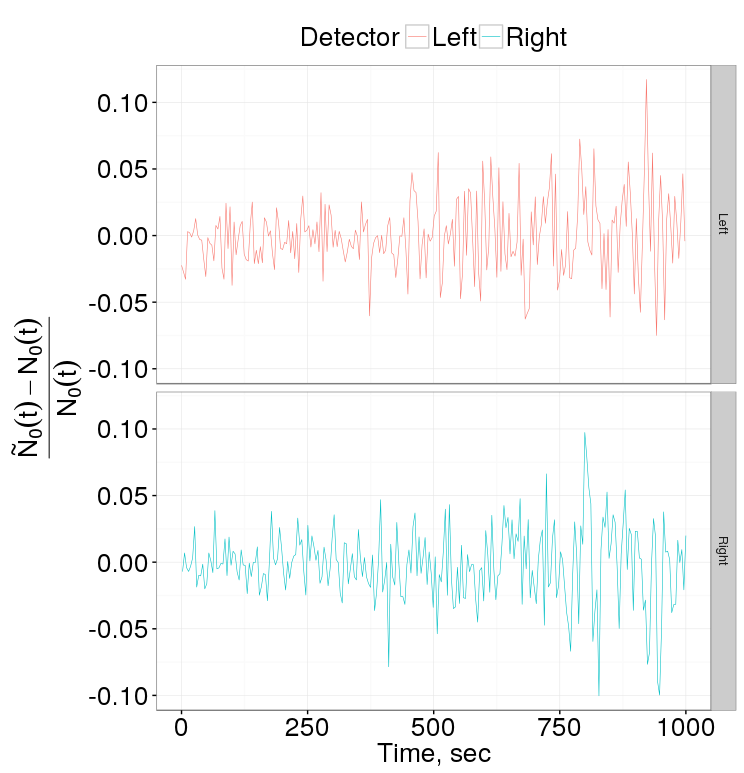
\includegraphics[width=\textwidth]{edm_img/LR_detector_relErr}
	\caption{Относительная ошибка измерения частоты событий на правом и левом
          детекторах как функция времени.\label{fig:LRDetErr}}
\end{figure}

\begin{figure}[H]
	\centering
	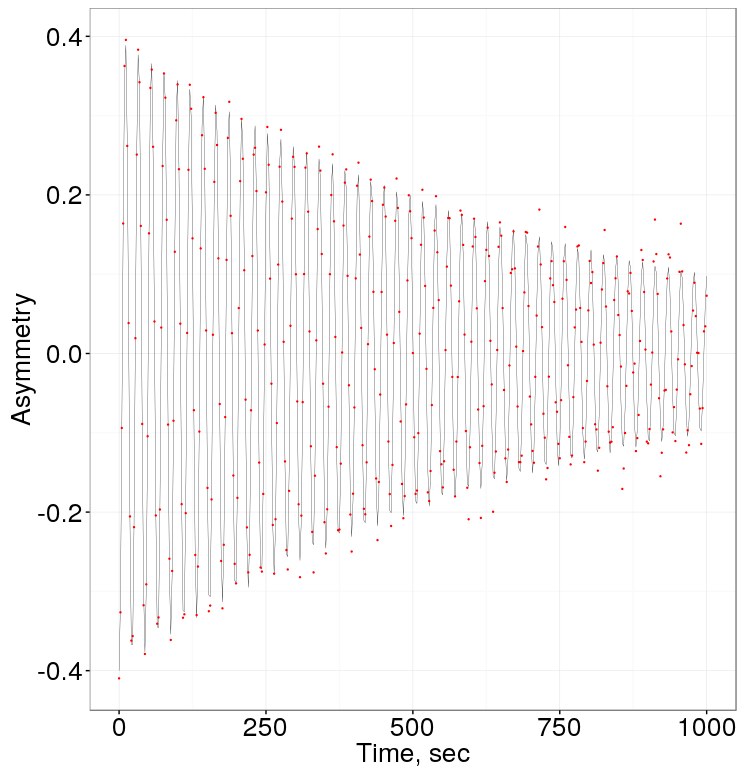
\includegraphics[width=\textwidth]{edm_img/Asymmetry}
	\caption{Ожидание (чёрная линия) и измерения (красные точки)
          асимметрии сечения.\label{fig:Asym}}
\end{figure}

Если начальная оценка частоты, полученная из равномерно собранного
сэмпла, имеет стандартную ошибку порядка $10^{-6}$ рад/сек, симуляции
подтверждают, что стандартная ошибка оценки может быть улучшена до примерно $\vp{5.8}{-7}$ рад/сек.

\section{Фальш-сигнал, связанный с неточностью установки магнитов}\label{sec:FalseSignalSim}
Данная серия симуляций была проведена с целью подтвердить два тезиса
касательно систематической ошибки измерения частоты прецессии спина в
вертикальной плоскости, вызванной неточностью установки E+B элементов:
\begin{inparaenum}[1)]
\item индуцированный МДМ-эффект зависит только от среднего значения
  угла наклона элементов, но не от  конкретной последовательности
  углов (т.е. отсутствует эффект \emph{геометрической фазы}); и
\item эта зависимость носит линейный характер.
\end{inparaenum}

Наклон элемента вокруг оптической оси моделировался путём добавления
после элемента спин-кика вокруг радиальной оси соответствующей
величины (см. раздел~\ref{sec:ErrorFieldImplementation}). Это
гарантирует сохранение замкнутой орбиты при введении наклонов, что
физически обусловлено появлением компенсирующего электрического поля 
спин-ротатора при его наклоне.

Симуляция была проведена следующим образом: мы распределили наклоны
$\Theta_{tilt}$ E+B элементам FS структуры случайным образом. После
построения матриц перехода 3-го порядка, были вычислены разложения
Тейлора функций спин-тюна и оси прецессии спина (SPA). Члены нулевого
порядка этих разложений представляют собой спин-тюн и SPA референсной частицы.

Симуляция была проведена 11 раз; каждый раз углы наклона
спин-ротаторов выбирались из нормального распределения
$N(\mu_0\cdot(i-5), \sigma_0)$, где $\mu_0 = 10\cdot \sigma_0 =
10^{-4}$ рад, $i\in\lbrace0,\dots, 10\rbrace$. Результаты представлены
на Рисунке~\ref{fig:Linearity_test_shifting_gauss}. На
Рисунке~\ref{fig:Linearity_test_compensated} показаны результаты,
когда три пары E+B повёрнуты на противоположные углы, а один повёрнут на угол
$\mu_i = (i-5)\cdot 10^{-6}$ рад,
$i\in\lbrace0,\dots,10\rbrace$. Симуляции были выполнены на энергии
270.0092 МэВ.\footnote{На этой энергии ось прецесии спина и спин-тюн
  не определены в системе координат связанной с пучком, использованной
  COSY INFINITY, для идеальной структуры. Это соответствует ситуации
  когда спин не прецессирует ни в какой плоскости (горизонтальной или
  вертикальной), что есть условие замороженного спина в идеальной структуре.}

\begin{figure}[H]
  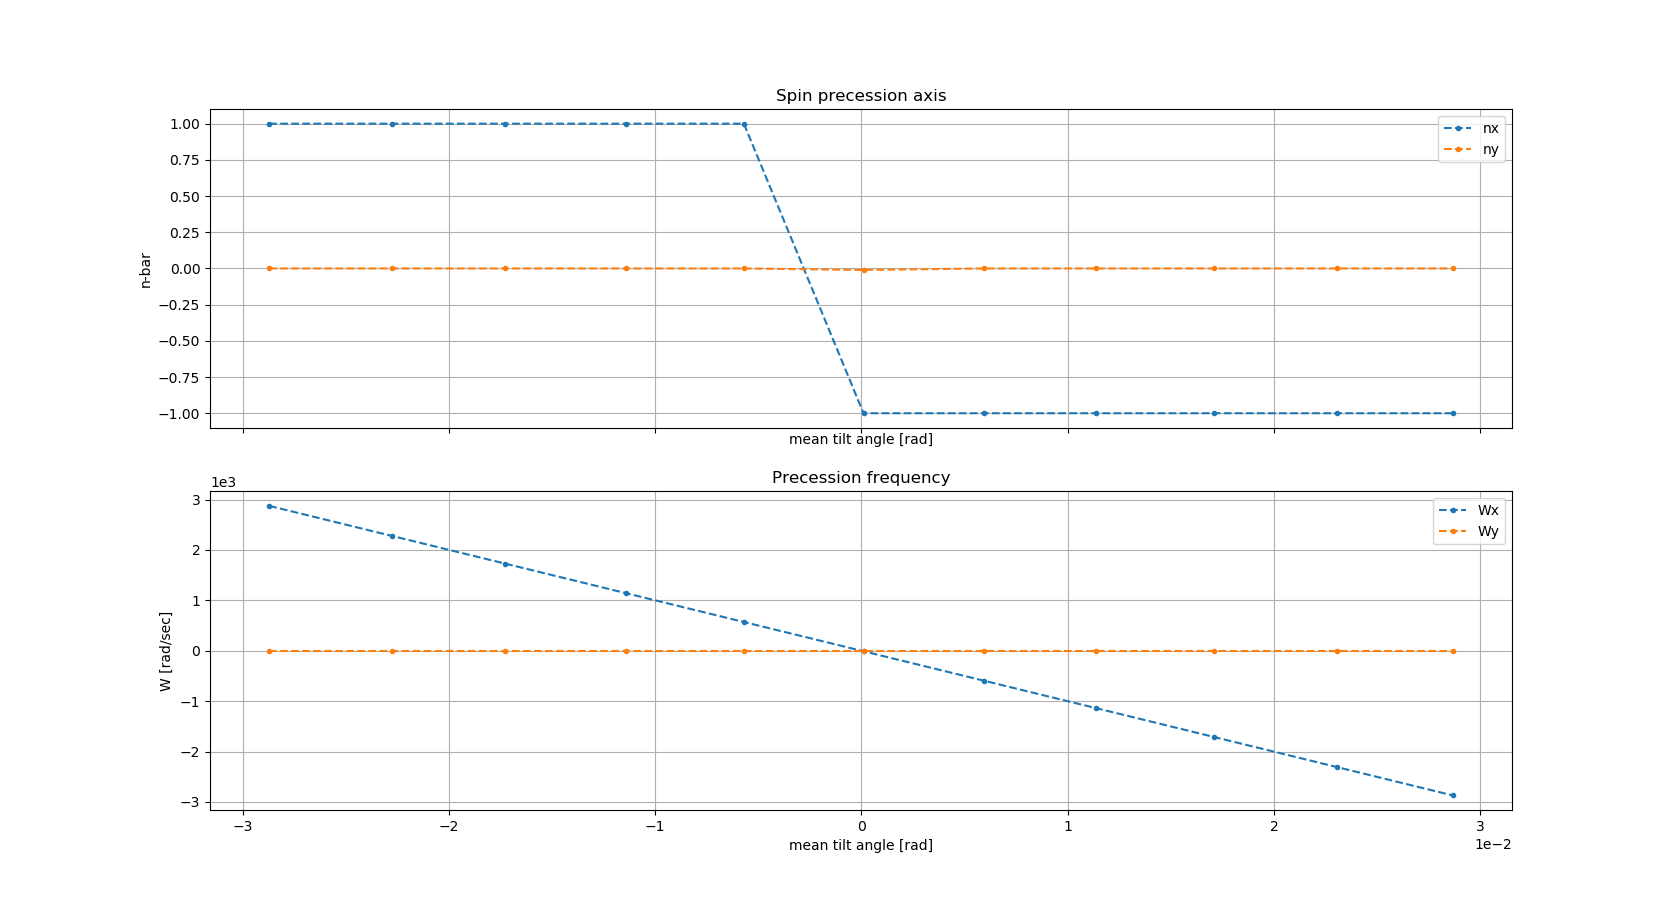
\includegraphics[width=\textwidth]{edm_img/linearity_test_shifting_gauss}
  \caption{Ось прецессии спина и частоты прецессии для неидеальной FS
    структуры, при наклонах E+B элементов.\label{fig:Linearity_test_shifting_gauss}}
\end{figure}
\begin{figure}[H]
  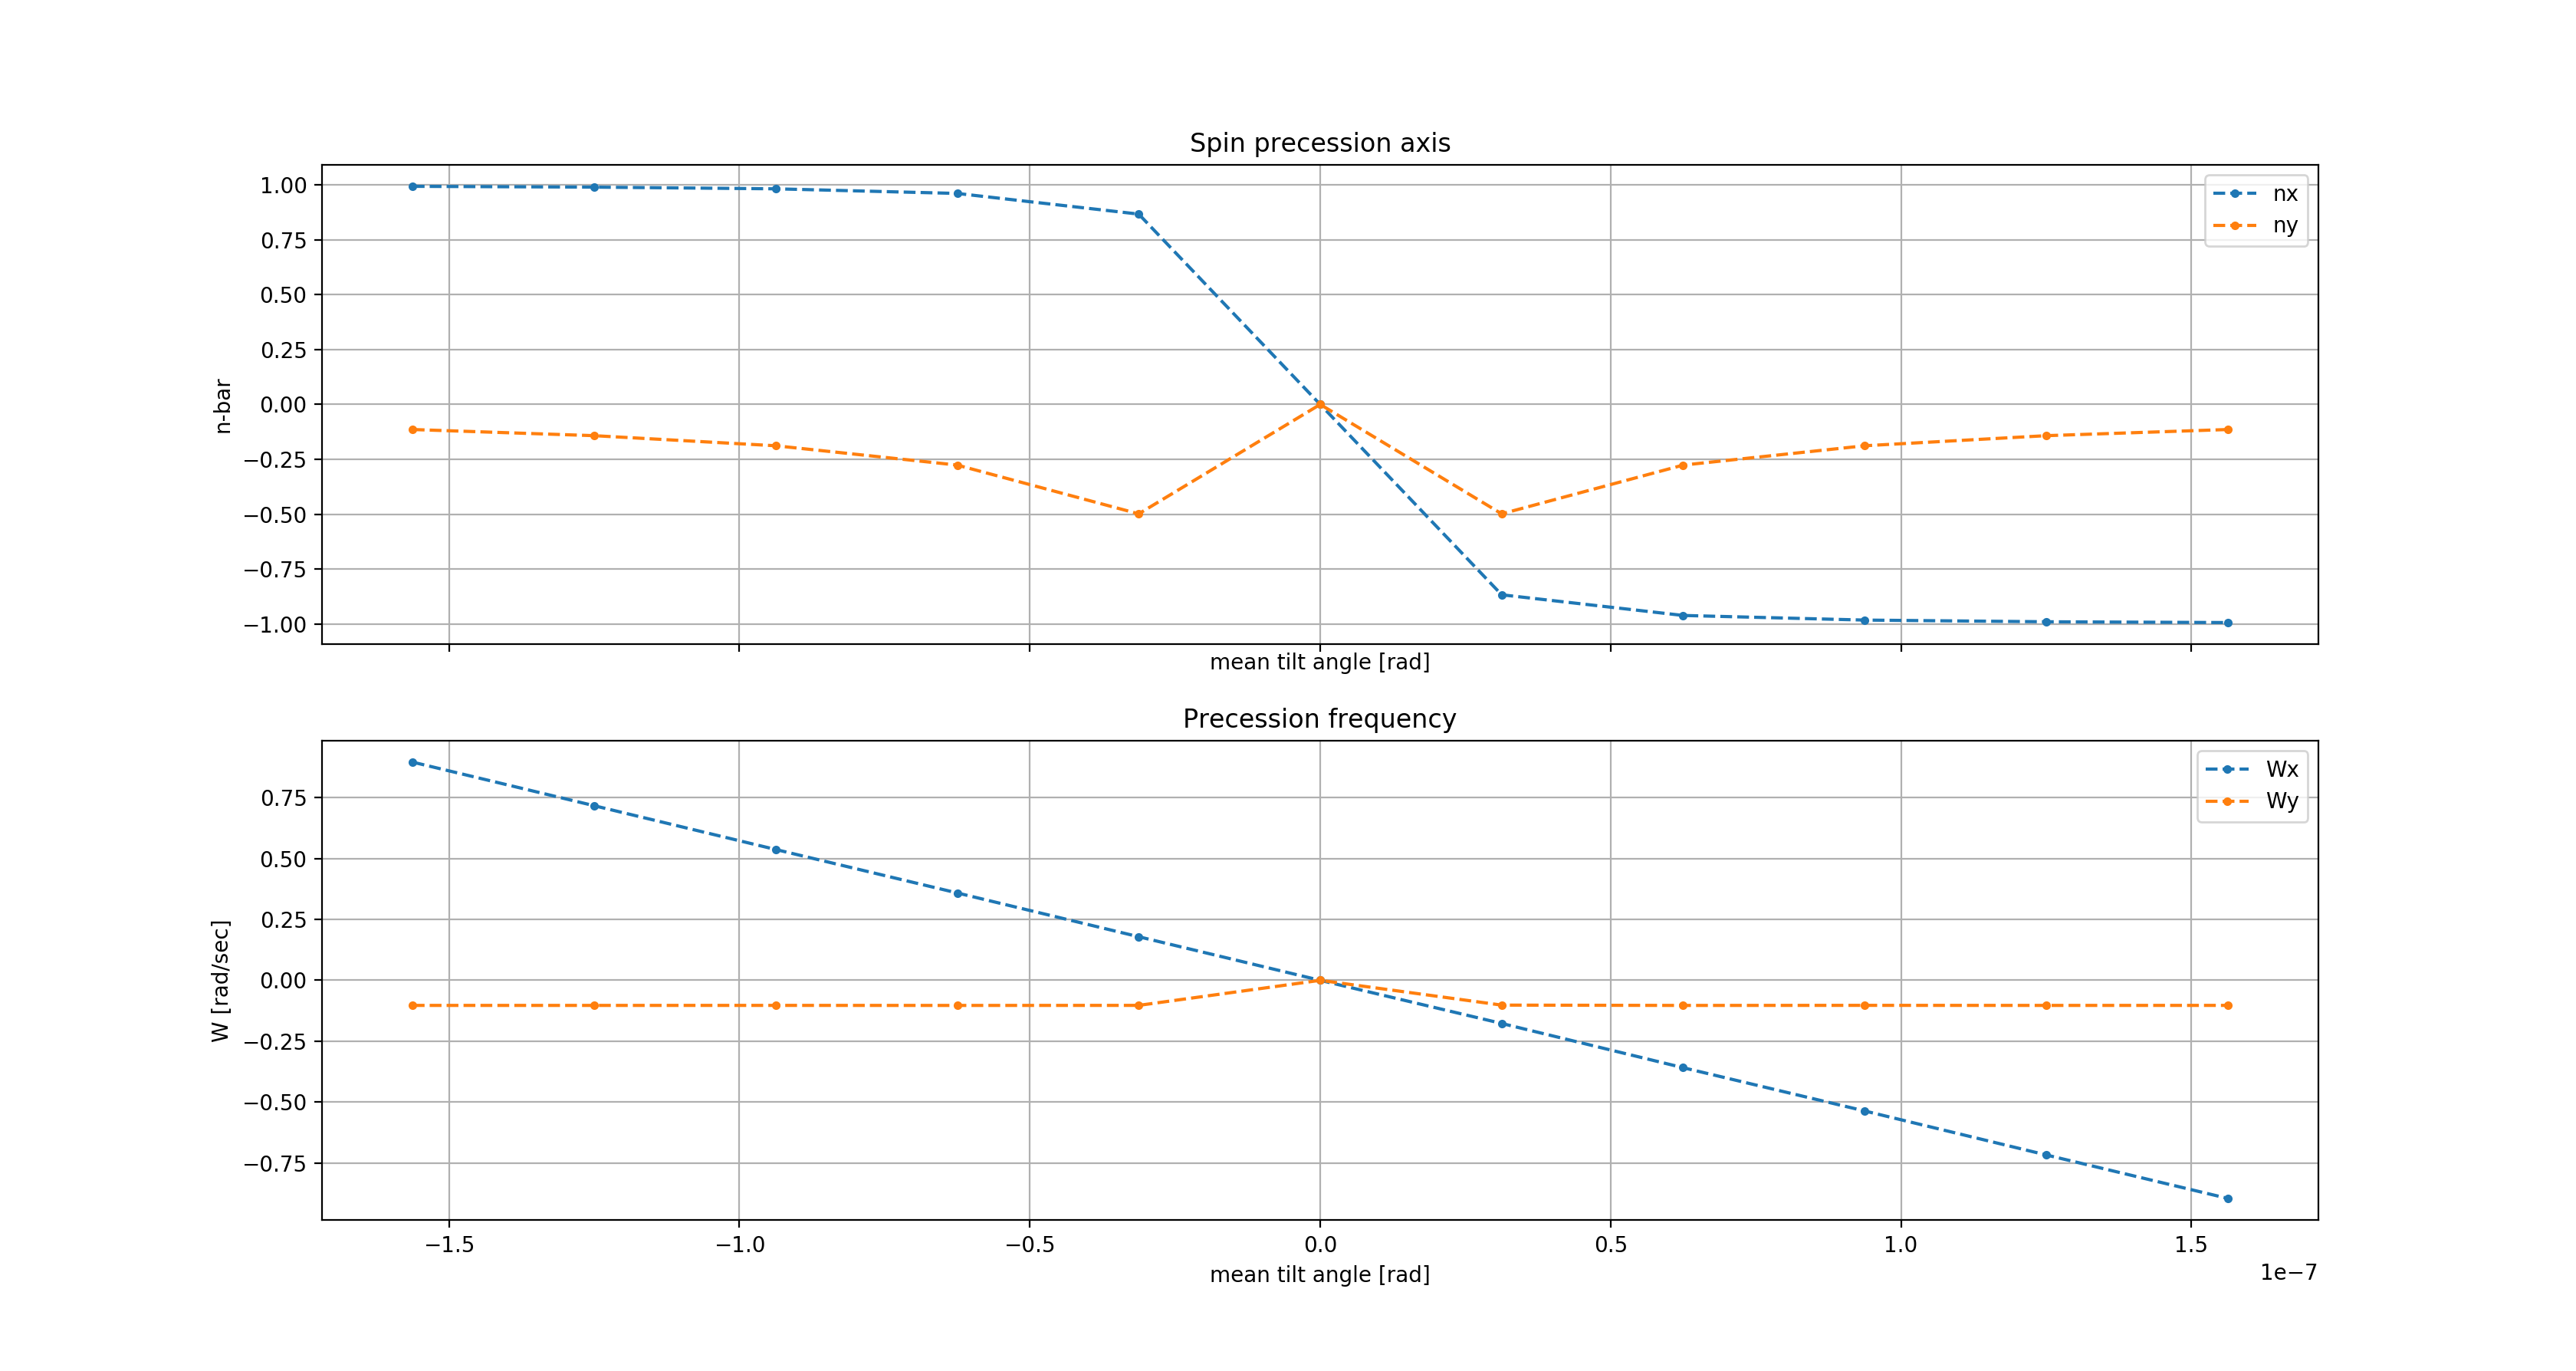
\includegraphics[width=\textwidth]{edm_img/linearity_test_compensated+microrad}
  \caption{Три пары противоположно наклонённых E+B элементов, плюс
    нескомпенсированный элемент.\label{fig:Linearity_test_compensated}}
\end{figure}


\section{Декогеренция}
При проведении нижеследующих тестов симулировалась инжекция
плоского, гауссовского пучка в структуру с замороженным
спином. Инжектируемые пучки состояли из 30 частиц, распределённых в
плоскости $y-z$ как $y\sim N(y_0, 10^{-4})$ [м]; $x,d =
0$. Оффсет $y_0$ варьировался в диапазоне $[-1, +1]$ мм. Начальное
направление спин-векторов всех частиц --- продольное: $\vec S(t=0) = (0,0,1)$.

Также в структуре варьировалось значение градиента GSY секступоля,
модулирующего декогеренцию в вертикальной плоскости. GSY менялся в
диапазоне $[GSY0 - 5\cdot10^{-3}, GSY0 + 5\cdot10^{-3}]$, где
$GSY0=-2.5e-3$ --- оптимальное значение градиента для идеальной структуры.

На каждое значение градиента приходится 10 инжекций.

Пучок инжектировался на энергии 270.0092 МэВ (строгий FS), в структуру
с неточно-установленными E+B спин-ротаторами. 

Наклоны E+B элементов
генерировались из распределения $N(0, 5\cdot10^{-4})$ радиан. При
симуляциях использовалась энергия строгой заморозки спина, а не,
например, близкая к ней 270 МэВ, для того, чтобы минимизировать
вертикальную компоненту оси прецессии. Матрицы перехода орбитального и спинового движений строятся до  третьего
порядка разложения ряда Тейлора, чтобы обеспечить устойчивость
процедуры TSS COSY Infinity.~\cite{COSYINF:BeamPhysMan}

Далее ансамбль начальных значений, представляющий пучок, трекается
через структуру на протяжении $1.2\cdot10^6$ оборотов, что
примерно эквивалентно 1.2 секундам. Каждые 800 оборотов производится
запись необходимых для анализа данных.

Собираемые данные: 
\begin{inparaenum}[\itshape a\upshape)]
\item результаты вычислений процедуры TSS: спин-тюн $\nu_s$ и компоненты вектора оси инвариантного спина
  $\bar n$, а также
\item компоненты спина $(S_X, S_Y, S_Z)$, и фазового пространства $(X,A,Y,B,T,D)$.
\end{inparaenum}

Из данных по компонентам спина вычисляется поляризация банча по
формуле
\[
\vec P = \frac{\sum_i\vec s_i}{|\sum_i\vec s_i|}.
\]

Поляризация фиритуется функцией $f(t; a,f,\phi) = a\cdot \sin(2\pi\cdot
f\cdot t + \phi)$, оцениваются все три параметра $(\hat a, \hat f,
\hat\phi)$. 

\subsection{Симуляция эффекта подавления декогеренции спина в вертикальной плоскости при помощи секступолей}
\begin{figure}[H]
  \centering
  \begin{subfigure}[b]{\textwidth}
    \includegraphics[width=\linewidth]{\multisext/ny_vs_offset}
    \caption{Вертикальная компонента оси прецессии спина $\bar n_y$ в зависимости
      от вертикального смещения центра пучка.\label{fig:DECOH_full_ny}}
  \end{subfigure}
\end{figure}
\begin{figure}[H]\ContinuedFloat
  \begin{subfigure}[b]{\textwidth}
    \includegraphics[width=\linewidth]{\multisext/ny_vs_offset_zoom}
    \caption{Деталировка Рисунка~\ref{fig:DECOH_full_ny}. Вертикальная компонента $\bar
      n_y$ (и $\bar n_x$) параболична вокруг референсной орбиты при
      оптимальном значении градиента GSY Y-секступоля, в отличии от
      $nu_s$, который линеен.}
  \end{subfigure}
\end{figure}
\begin{figure}[H]\ContinuedFloat
  \centering
  \begin{subfigure}[b]{\textwidth}
    \includegraphics[width=\linewidth]{\multisext/spin_tune_vs_offset}
    \caption{Спин-тюн $\nu_s$.}
  \end{subfigure}
  \caption{Данные DECOH построенные для каждого значения градиента GSY
    в зависимости от вертикального оффсета пучка.}
\end{figure}

\begin{figure}[H]
  \centering
  \begin{subfigure}[b]{\textwidth}
    \includegraphics[width=\linewidth]{\multisext/FreqY_vs_offset}
    \caption{Полный диапазон.\label{fig:FreqY_vs_offset}}
  \end{subfigure}
\end{figure}
\begin{figure}[H]\ContinuedFloat
  \begin{subfigure}[b]{\textwidth}
    \includegraphics[width=\linewidth]{\multisext/FreqY_vs_offset_zoom}
    \caption{Деталировка Рисунка~\ref{fig:FreqY_vs_offset}. Оценка
      частоты колебаний вертикальной компоненты поляризации зависит от
      начального оффсета пучка линейно, как спин-тюн $\nu_s$, а не как $\bar n_y$.}
  \end{subfigure}
  \caption{Оценка частоты прецессии поляризации пучка в вертикальной
    плоскости в зависимости от начального оффсета пучка от референсной
    орбиты для оптимального значения градиента GSY секступоля
    (оранжевый), и двух значений на противоположных концах
    рассматриваемого спектра значений GSY.}
\end{figure}

\subsection{Исследование зависимости оценки частоты прецессии поляризации банча от спин тюна и прецессии оси стабильного спина}\label{sec:SpinTune_and_SPA_dependence}

\begin{figure}[H]
  \centering
  \includegraphics[width=\linewidth]{\decoh/ny_vs_turn}
  \caption{Вертикальная компонента $\bar n$ для частиц с оффсетами,
    соответственно.: [1.02749, 1.02937, 1.02840] мм. Мы наблюдаем
    быстрые осцилляции вокруг некоторого среднего уровня. Этот средний
    уровень изменяется параболически с вертикальным оффсетом частиц
    (см. Рисунок~\ref{fig:mean_tune_axis} ниже). Быстрые осцилляции
    вызваны бетатронным движением (см. Рисунки~\ref{fig:tune_axis_position_y},~\ref{fig:tune_axis_position_x}).\label{fig:ny_vs_turn}}
\end{figure}
\begin{figure}[H]
	\centering
	\begin{subfigure}[b]{\textwidth}
		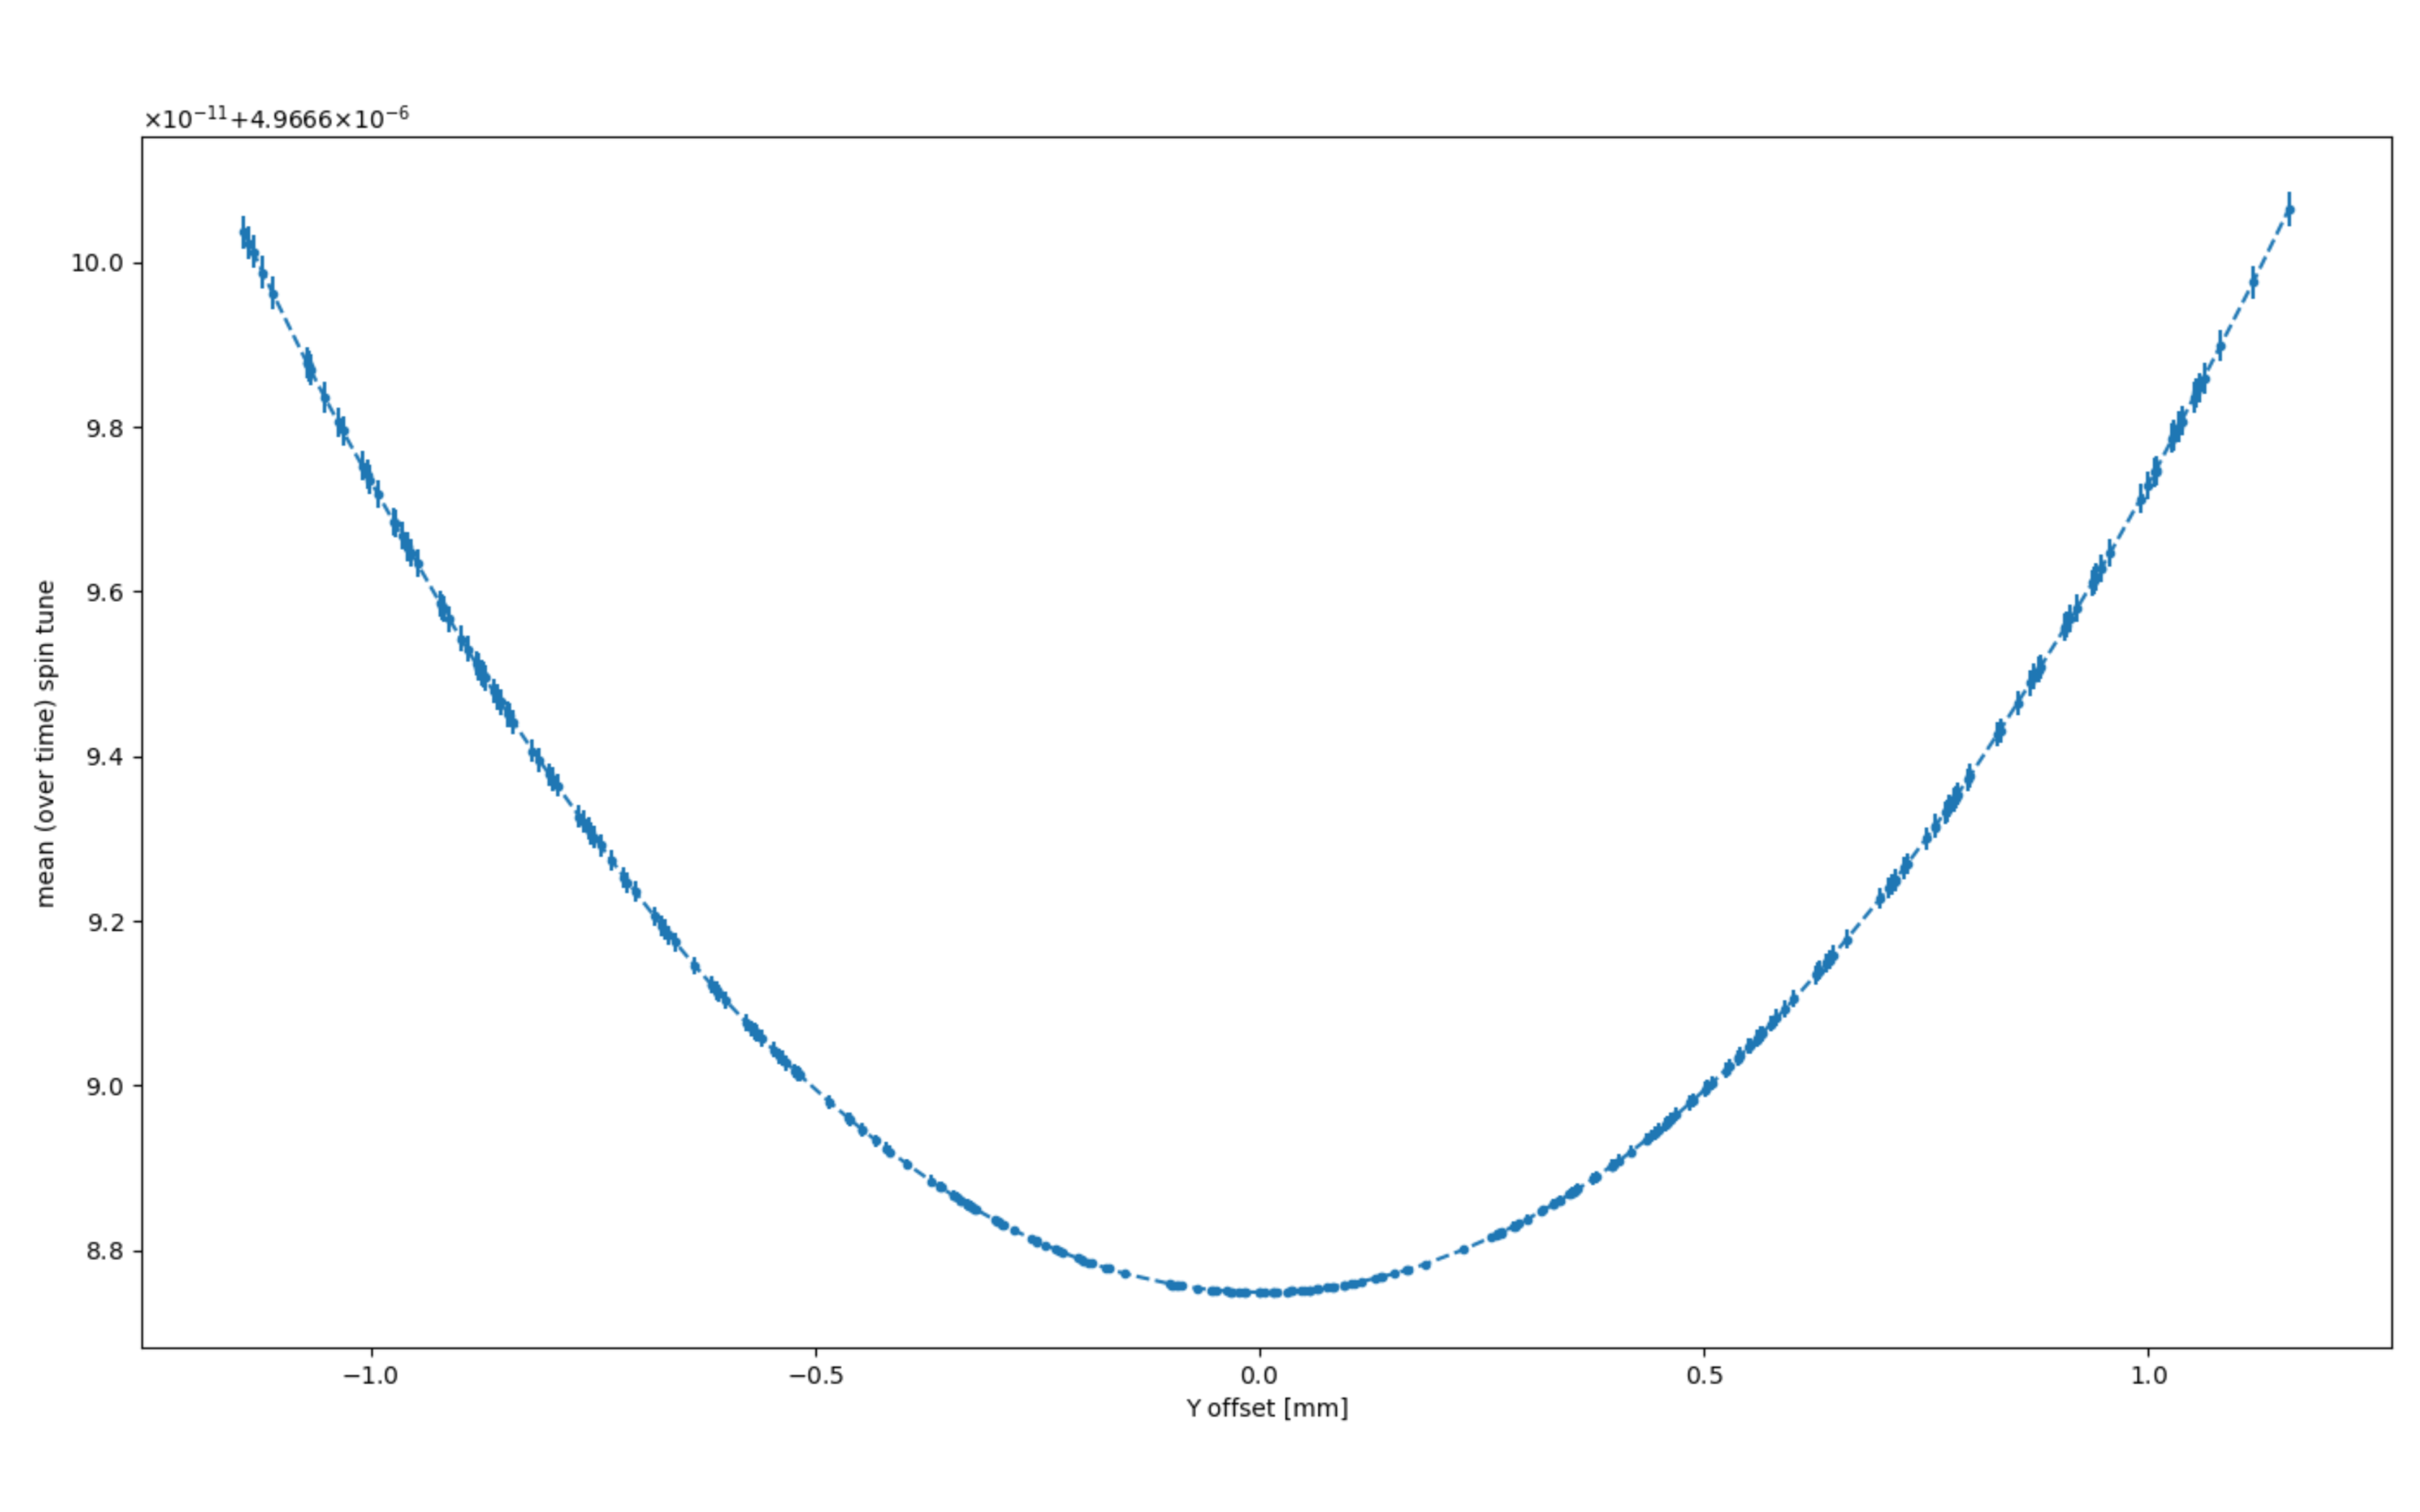
\includegraphics[width=\linewidth]{edm_img/mean_spin_tune_vs_y_offset}
		\caption{Средний уровень спин тюна в зависимости от вертикального сдвига пучка}
	\end{subfigure}

	\begin{subfigure}[b]{\textwidth}
		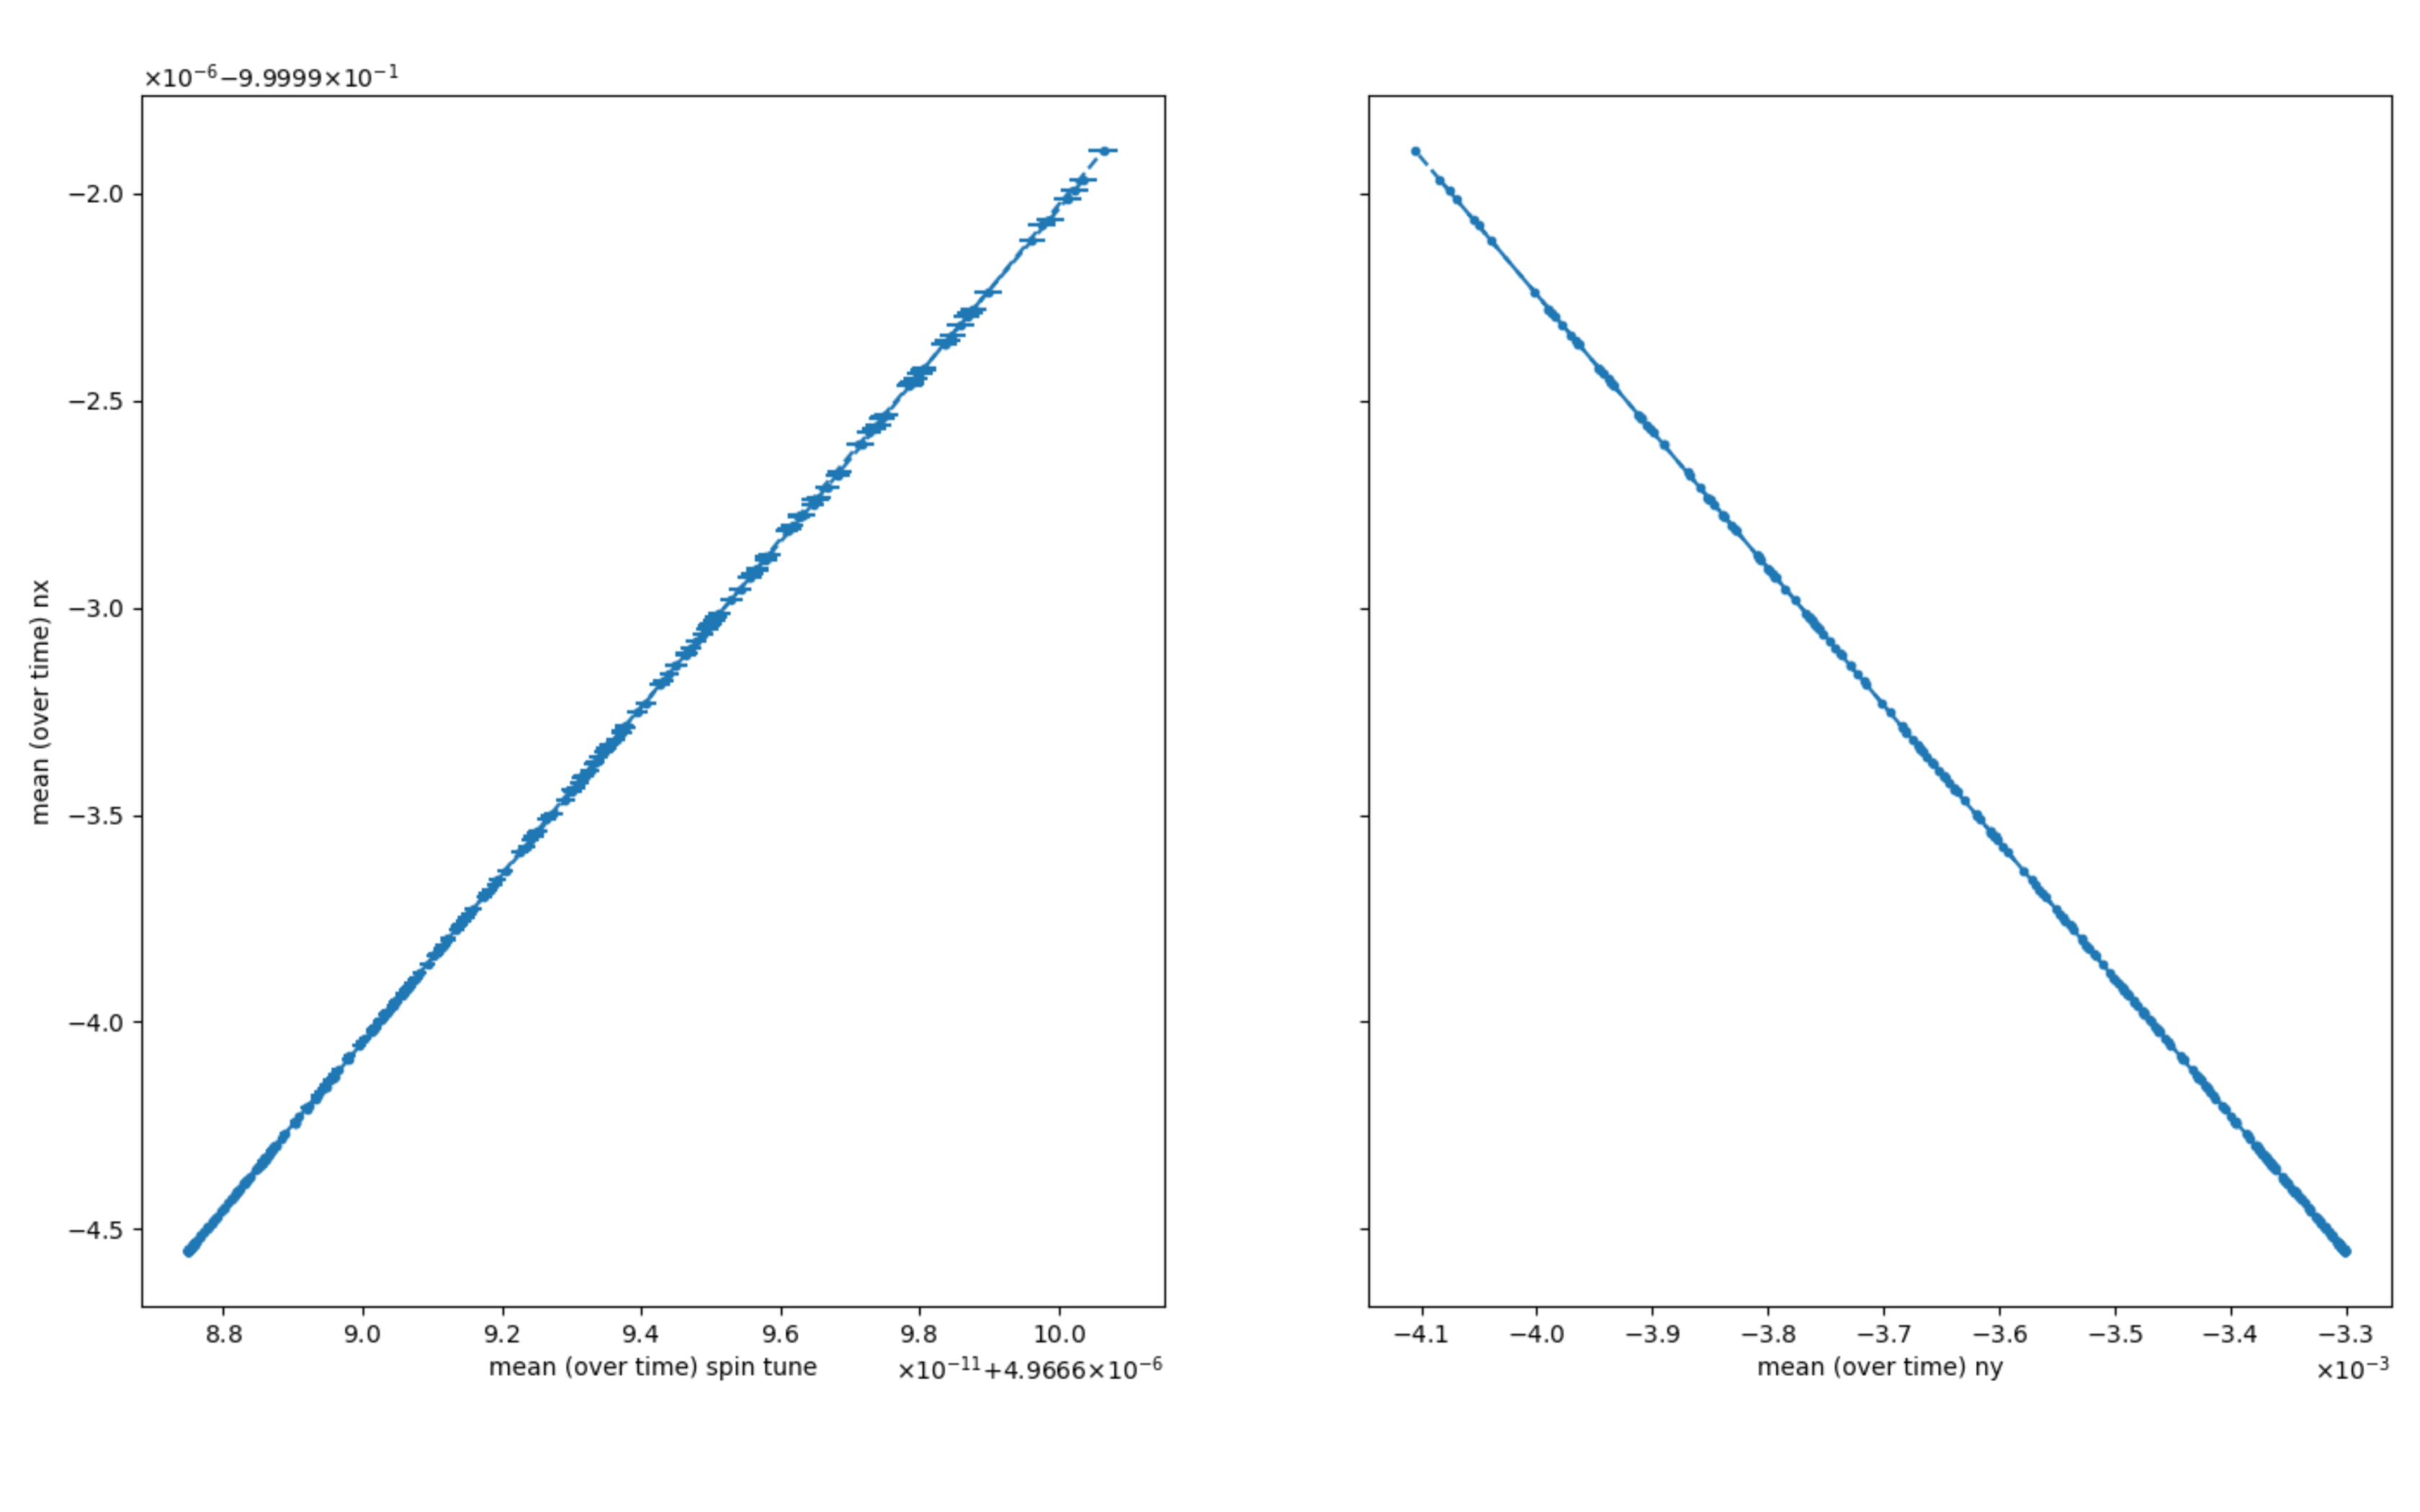
\includegraphics[width=\linewidth]{edm_img/mean_n_bar_vs_spin_tune}
		\caption{Связь средних уровней компонент $\bar n$ и спин тюна}
	\end{subfigure}
	\caption{Средние уровни спин тюна и оси стабильного спина в зависимости от начального вертикального сдвига пучка и друг друга. Видно, что спин тюн и ось прецессии спина жёстко связаны между собой.\label{fig:mean_tune_axis}}
\end{figure}

На Рисунке~\ref{fig:mean_tune_axis} видно, что средние уровни компонент оси прецессии спина связаны линейно со средним уровнем спин тюна; в связи с этим следует вывод, что использование секступольных полей выравнивает не только скорости вращения спинов частиц вокруг их собственных осей прецессии в некотором диапазоне вокруг замкнутой орбиты, но также и направления самих осей. 
\begin{figure}[H]
  \centering
  \begin{subfigure}[b]{\textwidth}
    \includegraphics[width=\linewidth]{\decoh/ny_vs_y}
    \caption{Вертикальная компонента $\bar n$ в зависимости от
      вертикального положения.}
  \end{subfigure}
\end{figure}
\begin{figure}[H]\ContinuedFloat
  \begin{subfigure}[b]{\textwidth}
    \includegraphics[width=\linewidth]{\decoh/spin_tune_vs_y}
    \caption{Спин-тюн в зависимости от вертикального положения.}
  \end{subfigure}
  \caption{Частота прецессии частицы в зависимости от её вертикального
    оффсета. Выраженная нефункциональность зависимости
    параметров от вертикального положения частицы, отражённая на
    рисунках --- следствие их зависимости также и от радиального положения
    частицы, которое также осциллирует на малой амплитуде (см. Рисунок~\ref{fig:tune_axis_position_x}). \label{fig:tune_axis_position_y}}
\end{figure}

\begin{figure}[H]
  \centering
  \begin{subfigure}[b]{\textwidth}
    \includegraphics[width=\linewidth]{\decoh/ny_vs_x}
    \caption{Вертикальная компонента $\bar n$ в зависимости от
      радиального положения.}
  \end{subfigure}

  \begin{subfigure}[b]{\textwidth}
    \includegraphics[width=\linewidth]{\decoh/spin_tune_vs_x}
    \caption{Спин-тюн в зависимости от радиального положения.}
  \end{subfigure}
  \caption{Частота прецессии спина в зависимости от радиального
    положения частицы.\label{fig:tune_axis_position_x}}
\end{figure}


\section{Калибровка величины ведущего магнитного поля с помощью
  частоты прецессии поляризации пучка в горизонтальной плоскости}
Симуляции и анализ данных по этому поводу ещё ведутся.

\chapter{Результаты обобщения и систематизации результатов проведённых исследований}

В процессе проведения работы было определено следующее:
\begin{enumerate}
	\item обоснованная длительность цикла измерений находится в диапазоне от двух до трёх постоянных времени жизни поляризации $\LTd$;
	\item при этом, статистически нет препятствий получению верхнего предела оценки ЭДМ дейтрона на уровне $10^{-29}~e\cdot cm$ за полное время измерений в один год;
	\item скорость паразитного МДМ вращения линейно зависит от среднего угла наклона спин-ротаторов, и не зависит от конкретной реализации распределения наклонов;
	\item при этом, величина этой скорости достаточно велика, чтобы сделать непрактичным оригинальный FS метод измерения ЭДМ;
	\item возможно использование секступольных полей для подавления декогеренции спина и, соответственно, увеличения времени жизни поляризации $\LTd$;
	\item использование секступольных полей одновременно выравнивает как скорости вращения спин-векторов частиц вокруг их собственных осей прецессии спина, так и направления самих этих осей, в некоторой области вокруг референсной орбиты;
	\item \emph{среднее} (по времени) направление оси прецессии спина частицы зависит от \emph{амплитуды} бетатронных колебаний, но не от конкретного положения частицы в поперечной плоскости вакуумной камеры.
\end{enumerate}

\chapter{Оценка достоверности и достаточности данных исследования}

На настоящий момент автор не понимает причину линейности связи между средними значениями спин-тюна и направления оси стабильного спина.  В следствии этого не ясен механизм выравнивания направления осей прецессии спинов частиц засчёт использования секступольных полей.

Также под сомнениями стоит возможность процедуры калибровки магнитного поля путём измерения частоты прецессии поляризации пучка в горизонтальной плоскости. Причина сомнений лежит в необходимости отведения энергии пучка от ``замороженного'' значения, и соответствующее изменение величины ведущего поля. Несмотря на возможность достаточно точной подстройки величины поля при помощи калибровки эффективного Лоренц-фактора на ``незамороженной'' энергии, при возвращении на ``замороженную'' энергию точность необходимо будет теряться.  Этой проблемы можно избежать, если производить калибровку поля не меняя энергию пучка, но тогда возникнет состояние ``замороженности'' спина во всех плоскостях, которое считается нестабильным.


\chapter{Заключения и выводы}
В данной работе, методами математического и численного моделирования исследован новый метод поиска электрического дипольного момента дейтрона с использованием комбинированного накопительного кольца. 

Изучено спин-орбитальное движение в кольцах, построенных на принципах ``замороженного'' и ``квази-замороженного'' спина. Проведено моделирование декогеренции прецессии спина, изучены методы её подавления с помощью мультипольных полей. Оценена систематическая ошибка методов измерения ЭДМ частиц в накопительном кольце, связанная с неточностью установки оптических элементов ускорителя. Изучен способ улучшения статистической погрешности оценки частоты колебаний вертикальной компоненты поляризации путём применения схемы временного модулирования измерений поляриметрии. 


\bibliography{\home/REPOS/EDM/Reports/PhD/PhDRefs}
\bibliographystyle{vancouver}

\end{document}
